% Created by tikzDevice version 0.12.6 on 2025-02-16 17:48:00
% !TEX encoding = UTF-8 Unicode
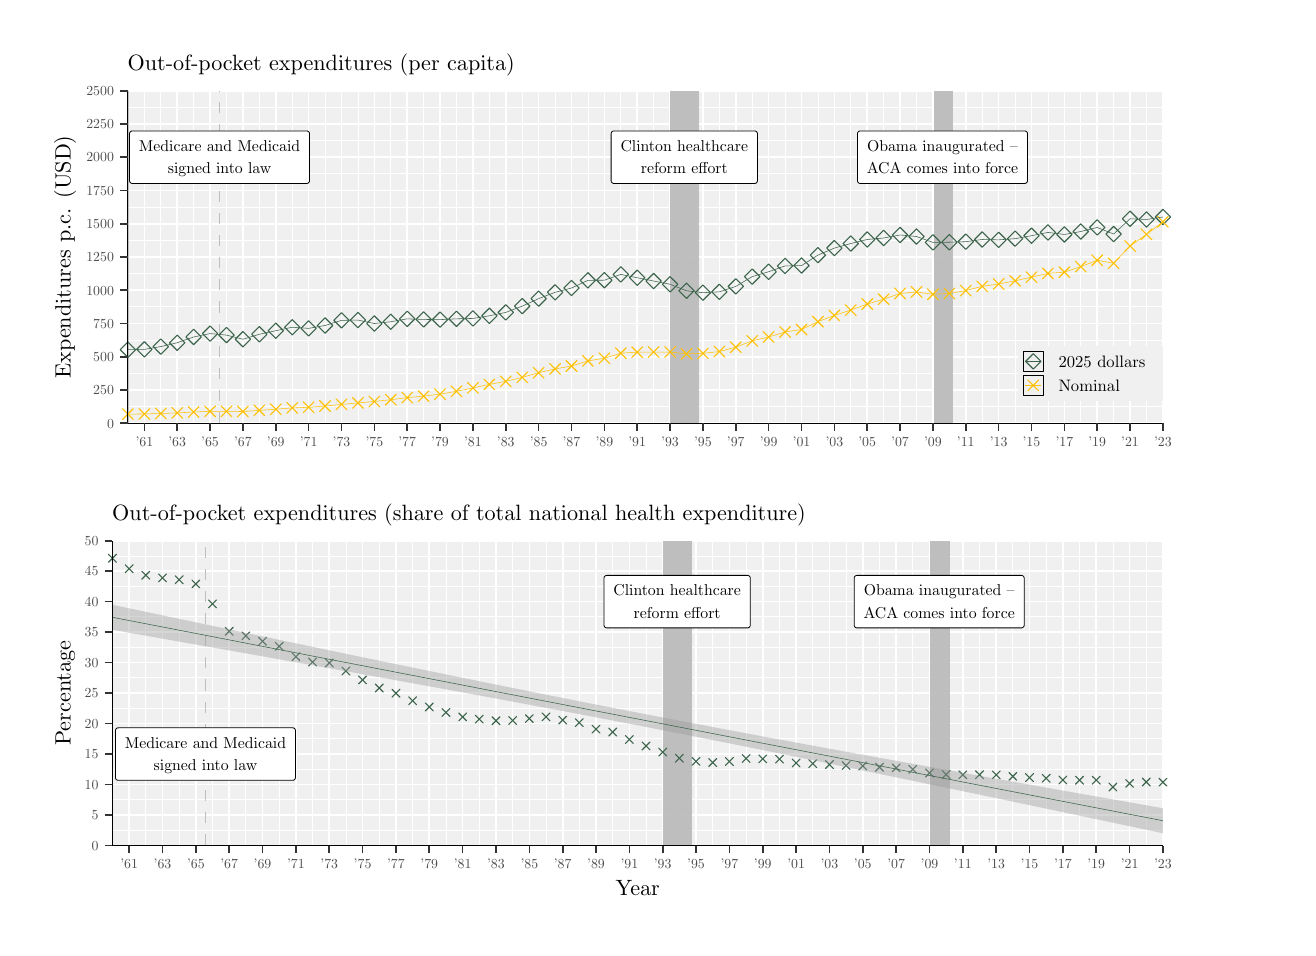
\begin{tikzpicture}[x=1pt,y=1pt]
\definecolor{fillColor}{RGB}{255,255,255}
\path[use as bounding box,fill=fillColor,fill opacity=0.00] (0,0) rectangle (455.30,325.21);
\begin{scope}
\path[clip] (  0.00,162.61) rectangle (455.30,325.21);
\definecolor{drawColor}{RGB}{255,255,255}
\definecolor{fillColor}{RGB}{255,255,255}

\path[draw=drawColor,line width= 0.6pt,line join=round,line cap=round,fill=fillColor] (  0.00,162.61) rectangle (455.30,325.21);
\end{scope}
\begin{scope}
\path[clip] (  0.00,  0.00) rectangle (455.30,325.21);
\definecolor{fillColor}{gray}{0.94}

\path[fill=fillColor] ( 36.14,182.27) rectangle (410.30,302.44);
\definecolor{drawColor}{RGB}{255,255,255}

\path[draw=drawColor,line width= 0.3pt,line join=round] ( 36.14,188.27) --
	(410.30,188.27);

\path[draw=drawColor,line width= 0.3pt,line join=round] ( 36.14,200.29) --
	(410.30,200.29);

\path[draw=drawColor,line width= 0.3pt,line join=round] ( 36.14,212.31) --
	(410.30,212.31);

\path[draw=drawColor,line width= 0.3pt,line join=round] ( 36.14,224.33) --
	(410.30,224.33);

\path[draw=drawColor,line width= 0.3pt,line join=round] ( 36.14,236.34) --
	(410.30,236.34);

\path[draw=drawColor,line width= 0.3pt,line join=round] ( 36.14,248.36) --
	(410.30,248.36);

\path[draw=drawColor,line width= 0.3pt,line join=round] ( 36.14,260.38) --
	(410.30,260.38);

\path[draw=drawColor,line width= 0.3pt,line join=round] ( 36.14,272.40) --
	(410.30,272.40);

\path[draw=drawColor,line width= 0.3pt,line join=round] ( 36.14,284.41) --
	(410.30,284.41);

\path[draw=drawColor,line width= 0.3pt,line join=round] ( 36.14,296.43) --
	(410.30,296.43);

\path[draw=drawColor,line width= 0.3pt,line join=round] ( 36.23,182.27) --
	( 36.23,302.44);

\path[draw=drawColor,line width= 0.3pt,line join=round] ( 48.10,182.27) --
	( 48.10,302.44);

\path[draw=drawColor,line width= 0.3pt,line join=round] ( 59.97,182.27) --
	( 59.97,302.44);

\path[draw=drawColor,line width= 0.3pt,line join=round] ( 71.85,182.27) --
	( 71.85,302.44);

\path[draw=drawColor,line width= 0.3pt,line join=round] ( 83.72,182.27) --
	( 83.72,302.44);

\path[draw=drawColor,line width= 0.3pt,line join=round] ( 95.59,182.27) --
	( 95.59,302.44);

\path[draw=drawColor,line width= 0.3pt,line join=round] (107.46,182.27) --
	(107.46,302.44);

\path[draw=drawColor,line width= 0.3pt,line join=round] (119.34,182.27) --
	(119.34,302.44);

\path[draw=drawColor,line width= 0.3pt,line join=round] (131.21,182.27) --
	(131.21,302.44);

\path[draw=drawColor,line width= 0.3pt,line join=round] (143.08,182.27) --
	(143.08,302.44);

\path[draw=drawColor,line width= 0.3pt,line join=round] (154.96,182.27) --
	(154.96,302.44);

\path[draw=drawColor,line width= 0.3pt,line join=round] (166.83,182.27) --
	(166.83,302.44);

\path[draw=drawColor,line width= 0.3pt,line join=round] (178.70,182.27) --
	(178.70,302.44);

\path[draw=drawColor,line width= 0.3pt,line join=round] (190.58,182.27) --
	(190.58,302.44);

\path[draw=drawColor,line width= 0.3pt,line join=round] (202.45,182.27) --
	(202.45,302.44);

\path[draw=drawColor,line width= 0.3pt,line join=round] (214.32,182.27) --
	(214.32,302.44);

\path[draw=drawColor,line width= 0.3pt,line join=round] (226.19,182.27) --
	(226.19,302.44);

\path[draw=drawColor,line width= 0.3pt,line join=round] (238.07,182.27) --
	(238.07,302.44);

\path[draw=drawColor,line width= 0.3pt,line join=round] (249.94,182.27) --
	(249.94,302.44);

\path[draw=drawColor,line width= 0.3pt,line join=round] (261.81,182.27) --
	(261.81,302.44);

\path[draw=drawColor,line width= 0.3pt,line join=round] (273.69,182.27) --
	(273.69,302.44);

\path[draw=drawColor,line width= 0.3pt,line join=round] (285.56,182.27) --
	(285.56,302.44);

\path[draw=drawColor,line width= 0.3pt,line join=round] (297.43,182.27) --
	(297.43,302.44);

\path[draw=drawColor,line width= 0.3pt,line join=round] (309.30,182.27) --
	(309.30,302.44);

\path[draw=drawColor,line width= 0.3pt,line join=round] (321.18,182.27) --
	(321.18,302.44);

\path[draw=drawColor,line width= 0.3pt,line join=round] (333.05,182.27) --
	(333.05,302.44);

\path[draw=drawColor,line width= 0.3pt,line join=round] (344.92,182.27) --
	(344.92,302.44);

\path[draw=drawColor,line width= 0.3pt,line join=round] (356.80,182.27) --
	(356.80,302.44);

\path[draw=drawColor,line width= 0.3pt,line join=round] (368.67,182.27) --
	(368.67,302.44);

\path[draw=drawColor,line width= 0.3pt,line join=round] (380.54,182.27) --
	(380.54,302.44);

\path[draw=drawColor,line width= 0.3pt,line join=round] (392.41,182.27) --
	(392.41,302.44);

\path[draw=drawColor,line width= 0.3pt,line join=round] (404.29,182.27) --
	(404.29,302.44);

\path[draw=drawColor,line width= 0.6pt,line join=round] ( 36.14,182.27) --
	(410.30,182.27);

\path[draw=drawColor,line width= 0.6pt,line join=round] ( 36.14,194.28) --
	(410.30,194.28);

\path[draw=drawColor,line width= 0.6pt,line join=round] ( 36.14,206.30) --
	(410.30,206.30);

\path[draw=drawColor,line width= 0.6pt,line join=round] ( 36.14,218.32) --
	(410.30,218.32);

\path[draw=drawColor,line width= 0.6pt,line join=round] ( 36.14,230.33) --
	(410.30,230.33);

\path[draw=drawColor,line width= 0.6pt,line join=round] ( 36.14,242.35) --
	(410.30,242.35);

\path[draw=drawColor,line width= 0.6pt,line join=round] ( 36.14,254.37) --
	(410.30,254.37);

\path[draw=drawColor,line width= 0.6pt,line join=round] ( 36.14,266.39) --
	(410.30,266.39);

\path[draw=drawColor,line width= 0.6pt,line join=round] ( 36.14,278.40) --
	(410.30,278.40);

\path[draw=drawColor,line width= 0.6pt,line join=round] ( 36.14,290.42) --
	(410.30,290.42);

\path[draw=drawColor,line width= 0.6pt,line join=round] ( 36.14,302.44) --
	(410.30,302.44);

\path[draw=drawColor,line width= 0.6pt,line join=round] ( 42.17,182.27) --
	( 42.17,302.44);

\path[draw=drawColor,line width= 0.6pt,line join=round] ( 54.03,182.27) --
	( 54.03,302.44);

\path[draw=drawColor,line width= 0.6pt,line join=round] ( 65.91,182.27) --
	( 65.91,302.44);

\path[draw=drawColor,line width= 0.6pt,line join=round] ( 77.78,182.27) --
	( 77.78,302.44);

\path[draw=drawColor,line width= 0.6pt,line join=round] ( 89.66,182.27) --
	( 89.66,302.44);

\path[draw=drawColor,line width= 0.6pt,line join=round] (101.52,182.27) --
	(101.52,302.44);

\path[draw=drawColor,line width= 0.6pt,line join=round] (113.41,182.27) --
	(113.41,302.44);

\path[draw=drawColor,line width= 0.6pt,line join=round] (125.27,182.27) --
	(125.27,302.44);

\path[draw=drawColor,line width= 0.6pt,line join=round] (137.15,182.27) --
	(137.15,302.44);

\path[draw=drawColor,line width= 0.6pt,line join=round] (149.02,182.27) --
	(149.02,302.44);

\path[draw=drawColor,line width= 0.6pt,line join=round] (160.90,182.27) --
	(160.90,302.44);

\path[draw=drawColor,line width= 0.6pt,line join=round] (172.76,182.27) --
	(172.76,302.44);

\path[draw=drawColor,line width= 0.6pt,line join=round] (184.64,182.27) --
	(184.64,302.44);

\path[draw=drawColor,line width= 0.6pt,line join=round] (196.51,182.27) --
	(196.51,302.44);

\path[draw=drawColor,line width= 0.6pt,line join=round] (208.39,182.27) --
	(208.39,302.44);

\path[draw=drawColor,line width= 0.6pt,line join=round] (220.25,182.27) --
	(220.25,302.44);

\path[draw=drawColor,line width= 0.6pt,line join=round] (232.13,182.27) --
	(232.13,302.44);

\path[draw=drawColor,line width= 0.6pt,line join=round] (244.00,182.27) --
	(244.00,302.44);

\path[draw=drawColor,line width= 0.6pt,line join=round] (255.88,182.27) --
	(255.88,302.44);

\path[draw=drawColor,line width= 0.6pt,line join=round] (267.74,182.27) --
	(267.74,302.44);

\path[draw=drawColor,line width= 0.6pt,line join=round] (279.63,182.27) --
	(279.63,302.44);

\path[draw=drawColor,line width= 0.6pt,line join=round] (291.49,182.27) --
	(291.49,302.44);

\path[draw=drawColor,line width= 0.6pt,line join=round] (303.37,182.27) --
	(303.37,302.44);

\path[draw=drawColor,line width= 0.6pt,line join=round] (315.24,182.27) --
	(315.24,302.44);

\path[draw=drawColor,line width= 0.6pt,line join=round] (327.12,182.27) --
	(327.12,302.44);

\path[draw=drawColor,line width= 0.6pt,line join=round] (338.98,182.27) --
	(338.98,302.44);

\path[draw=drawColor,line width= 0.6pt,line join=round] (350.86,182.27) --
	(350.86,302.44);

\path[draw=drawColor,line width= 0.6pt,line join=round] (362.73,182.27) --
	(362.73,302.44);

\path[draw=drawColor,line width= 0.6pt,line join=round] (374.61,182.27) --
	(374.61,302.44);

\path[draw=drawColor,line width= 0.6pt,line join=round] (386.47,182.27) --
	(386.47,302.44);

\path[draw=drawColor,line width= 0.6pt,line join=round] (398.35,182.27) --
	(398.35,302.44);

\path[draw=drawColor,line width= 0.6pt,line join=round] (410.22,182.27) --
	(410.22,302.44);
\definecolor{drawColor}{RGB}{190,190,190}

\path[draw=drawColor,line width= 0.6pt,line join=round] ( 36.22,182.27) -- ( 36.22,302.44);
\definecolor{fillColor}{RGB}{190,190,190}

\path[fill=fillColor,fill opacity=0.01] (232.13,182.27) rectangle (242.42,302.44);

\path[fill=fillColor,fill opacity=0.01] (232.13,182.27) rectangle (242.42,302.44);

\path[fill=fillColor,fill opacity=0.01] (232.13,182.27) rectangle (242.42,302.44);

\path[fill=fillColor,fill opacity=0.01] (232.13,182.27) rectangle (242.42,302.44);

\path[fill=fillColor,fill opacity=0.01] (232.13,182.27) rectangle (242.42,302.44);

\path[fill=fillColor,fill opacity=0.01] (232.13,182.27) rectangle (242.42,302.44);

\path[fill=fillColor,fill opacity=0.01] (232.13,182.27) rectangle (242.42,302.44);

\path[fill=fillColor,fill opacity=0.01] (232.13,182.27) rectangle (242.42,302.44);

\path[fill=fillColor,fill opacity=0.01] (232.13,182.27) rectangle (242.42,302.44);

\path[fill=fillColor,fill opacity=0.01] (232.13,182.27) rectangle (242.42,302.44);

\path[fill=fillColor,fill opacity=0.01] (232.13,182.27) rectangle (242.42,302.44);

\path[fill=fillColor,fill opacity=0.01] (232.13,182.27) rectangle (242.42,302.44);

\path[fill=fillColor,fill opacity=0.01] (232.13,182.27) rectangle (242.42,302.44);

\path[fill=fillColor,fill opacity=0.01] (232.13,182.27) rectangle (242.42,302.44);

\path[fill=fillColor,fill opacity=0.01] (232.13,182.27) rectangle (242.42,302.44);

\path[fill=fillColor,fill opacity=0.01] (232.13,182.27) rectangle (242.42,302.44);

\path[fill=fillColor,fill opacity=0.01] (232.13,182.27) rectangle (242.42,302.44);

\path[fill=fillColor,fill opacity=0.01] (232.13,182.27) rectangle (242.42,302.44);

\path[fill=fillColor,fill opacity=0.01] (232.13,182.27) rectangle (242.42,302.44);

\path[fill=fillColor,fill opacity=0.01] (232.13,182.27) rectangle (242.42,302.44);

\path[fill=fillColor,fill opacity=0.01] (232.13,182.27) rectangle (242.42,302.44);

\path[fill=fillColor,fill opacity=0.01] (232.13,182.27) rectangle (242.42,302.44);

\path[fill=fillColor,fill opacity=0.01] (232.13,182.27) rectangle (242.42,302.44);

\path[fill=fillColor,fill opacity=0.01] (232.13,182.27) rectangle (242.42,302.44);

\path[fill=fillColor,fill opacity=0.01] (232.13,182.27) rectangle (242.42,302.44);

\path[fill=fillColor,fill opacity=0.01] (232.13,182.27) rectangle (242.42,302.44);

\path[fill=fillColor,fill opacity=0.01] (232.13,182.27) rectangle (242.42,302.44);

\path[fill=fillColor,fill opacity=0.01] (232.13,182.27) rectangle (242.42,302.44);

\path[fill=fillColor,fill opacity=0.01] (232.13,182.27) rectangle (242.42,302.44);

\path[fill=fillColor,fill opacity=0.01] (232.13,182.27) rectangle (242.42,302.44);

\path[fill=fillColor,fill opacity=0.01] (232.13,182.27) rectangle (242.42,302.44);

\path[fill=fillColor,fill opacity=0.01] (232.13,182.27) rectangle (242.42,302.44);

\path[fill=fillColor,fill opacity=0.01] (232.13,182.27) rectangle (242.42,302.44);

\path[fill=fillColor,fill opacity=0.01] (232.13,182.27) rectangle (242.42,302.44);

\path[fill=fillColor,fill opacity=0.01] (232.13,182.27) rectangle (242.42,302.44);

\path[fill=fillColor,fill opacity=0.01] (232.13,182.27) rectangle (242.42,302.44);

\path[fill=fillColor,fill opacity=0.01] (232.13,182.27) rectangle (242.42,302.44);

\path[fill=fillColor,fill opacity=0.01] (232.13,182.27) rectangle (242.42,302.44);

\path[fill=fillColor,fill opacity=0.01] (232.13,182.27) rectangle (242.42,302.44);

\path[fill=fillColor,fill opacity=0.01] (232.13,182.27) rectangle (242.42,302.44);

\path[fill=fillColor,fill opacity=0.01] (232.13,182.27) rectangle (242.42,302.44);

\path[fill=fillColor,fill opacity=0.01] (232.13,182.27) rectangle (242.42,302.44);

\path[fill=fillColor,fill opacity=0.01] (232.13,182.27) rectangle (242.42,302.44);

\path[fill=fillColor,fill opacity=0.01] (232.13,182.27) rectangle (242.42,302.44);

\path[fill=fillColor,fill opacity=0.01] (232.13,182.27) rectangle (242.42,302.44);

\path[fill=fillColor,fill opacity=0.01] (232.13,182.27) rectangle (242.42,302.44);

\path[fill=fillColor,fill opacity=0.01] (232.13,182.27) rectangle (242.42,302.44);

\path[fill=fillColor,fill opacity=0.01] (232.13,182.27) rectangle (242.42,302.44);

\path[fill=fillColor,fill opacity=0.01] (232.13,182.27) rectangle (242.42,302.44);

\path[fill=fillColor,fill opacity=0.01] (232.13,182.27) rectangle (242.42,302.44);

\path[fill=fillColor,fill opacity=0.01] (232.13,182.27) rectangle (242.42,302.44);

\path[fill=fillColor,fill opacity=0.01] (232.13,182.27) rectangle (242.42,302.44);

\path[fill=fillColor,fill opacity=0.01] (232.13,182.27) rectangle (242.42,302.44);

\path[fill=fillColor,fill opacity=0.01] (232.13,182.27) rectangle (242.42,302.44);

\path[fill=fillColor,fill opacity=0.01] (232.13,182.27) rectangle (242.42,302.44);

\path[fill=fillColor,fill opacity=0.01] (232.13,182.27) rectangle (242.42,302.44);

\path[fill=fillColor,fill opacity=0.01] (232.13,182.27) rectangle (242.42,302.44);

\path[fill=fillColor,fill opacity=0.01] (232.13,182.27) rectangle (242.42,302.44);

\path[fill=fillColor,fill opacity=0.01] (232.13,182.27) rectangle (242.42,302.44);

\path[fill=fillColor,fill opacity=0.01] (232.13,182.27) rectangle (242.42,302.44);

\path[fill=fillColor,fill opacity=0.01] (232.13,182.27) rectangle (242.42,302.44);

\path[fill=fillColor,fill opacity=0.01] (232.13,182.27) rectangle (242.42,302.44);

\path[fill=fillColor,fill opacity=0.01] (232.13,182.27) rectangle (242.42,302.44);

\path[fill=fillColor,fill opacity=0.01] (232.13,182.27) rectangle (242.42,302.44);

\path[fill=fillColor,fill opacity=0.01] (327.43,182.27) rectangle (334.37,302.44);

\path[fill=fillColor,fill opacity=0.01] (327.43,182.27) rectangle (334.37,302.44);

\path[fill=fillColor,fill opacity=0.01] (327.43,182.27) rectangle (334.37,302.44);

\path[fill=fillColor,fill opacity=0.01] (327.43,182.27) rectangle (334.37,302.44);

\path[fill=fillColor,fill opacity=0.01] (327.43,182.27) rectangle (334.37,302.44);

\path[fill=fillColor,fill opacity=0.01] (327.43,182.27) rectangle (334.37,302.44);

\path[fill=fillColor,fill opacity=0.01] (327.43,182.27) rectangle (334.37,302.44);

\path[fill=fillColor,fill opacity=0.01] (327.43,182.27) rectangle (334.37,302.44);

\path[fill=fillColor,fill opacity=0.01] (327.43,182.27) rectangle (334.37,302.44);

\path[fill=fillColor,fill opacity=0.01] (327.43,182.27) rectangle (334.37,302.44);

\path[fill=fillColor,fill opacity=0.01] (327.43,182.27) rectangle (334.37,302.44);

\path[fill=fillColor,fill opacity=0.01] (327.43,182.27) rectangle (334.37,302.44);

\path[fill=fillColor,fill opacity=0.01] (327.43,182.27) rectangle (334.37,302.44);

\path[fill=fillColor,fill opacity=0.01] (327.43,182.27) rectangle (334.37,302.44);

\path[fill=fillColor,fill opacity=0.01] (327.43,182.27) rectangle (334.37,302.44);

\path[fill=fillColor,fill opacity=0.01] (327.43,182.27) rectangle (334.37,302.44);

\path[fill=fillColor,fill opacity=0.01] (327.43,182.27) rectangle (334.37,302.44);

\path[fill=fillColor,fill opacity=0.01] (327.43,182.27) rectangle (334.37,302.44);

\path[fill=fillColor,fill opacity=0.01] (327.43,182.27) rectangle (334.37,302.44);

\path[fill=fillColor,fill opacity=0.01] (327.43,182.27) rectangle (334.37,302.44);

\path[fill=fillColor,fill opacity=0.01] (327.43,182.27) rectangle (334.37,302.44);

\path[fill=fillColor,fill opacity=0.01] (327.43,182.27) rectangle (334.37,302.44);

\path[fill=fillColor,fill opacity=0.01] (327.43,182.27) rectangle (334.37,302.44);

\path[fill=fillColor,fill opacity=0.01] (327.43,182.27) rectangle (334.37,302.44);

\path[fill=fillColor,fill opacity=0.01] (327.43,182.27) rectangle (334.37,302.44);

\path[fill=fillColor,fill opacity=0.01] (327.43,182.27) rectangle (334.37,302.44);

\path[fill=fillColor,fill opacity=0.01] (327.43,182.27) rectangle (334.37,302.44);

\path[fill=fillColor,fill opacity=0.01] (327.43,182.27) rectangle (334.37,302.44);

\path[fill=fillColor,fill opacity=0.01] (327.43,182.27) rectangle (334.37,302.44);

\path[fill=fillColor,fill opacity=0.01] (327.43,182.27) rectangle (334.37,302.44);

\path[fill=fillColor,fill opacity=0.01] (327.43,182.27) rectangle (334.37,302.44);

\path[fill=fillColor,fill opacity=0.01] (327.43,182.27) rectangle (334.37,302.44);

\path[fill=fillColor,fill opacity=0.01] (327.43,182.27) rectangle (334.37,302.44);

\path[fill=fillColor,fill opacity=0.01] (327.43,182.27) rectangle (334.37,302.44);

\path[fill=fillColor,fill opacity=0.01] (327.43,182.27) rectangle (334.37,302.44);

\path[fill=fillColor,fill opacity=0.01] (327.43,182.27) rectangle (334.37,302.44);

\path[fill=fillColor,fill opacity=0.01] (327.43,182.27) rectangle (334.37,302.44);

\path[fill=fillColor,fill opacity=0.01] (327.43,182.27) rectangle (334.37,302.44);

\path[fill=fillColor,fill opacity=0.01] (327.43,182.27) rectangle (334.37,302.44);

\path[fill=fillColor,fill opacity=0.01] (327.43,182.27) rectangle (334.37,302.44);

\path[fill=fillColor,fill opacity=0.01] (327.43,182.27) rectangle (334.37,302.44);

\path[fill=fillColor,fill opacity=0.01] (327.43,182.27) rectangle (334.37,302.44);

\path[fill=fillColor,fill opacity=0.01] (327.43,182.27) rectangle (334.37,302.44);

\path[fill=fillColor,fill opacity=0.01] (327.43,182.27) rectangle (334.37,302.44);

\path[fill=fillColor,fill opacity=0.01] (327.43,182.27) rectangle (334.37,302.44);

\path[fill=fillColor,fill opacity=0.01] (327.43,182.27) rectangle (334.37,302.44);

\path[fill=fillColor,fill opacity=0.01] (327.43,182.27) rectangle (334.37,302.44);

\path[fill=fillColor,fill opacity=0.01] (327.43,182.27) rectangle (334.37,302.44);

\path[fill=fillColor,fill opacity=0.01] (327.43,182.27) rectangle (334.37,302.44);

\path[fill=fillColor,fill opacity=0.01] (327.43,182.27) rectangle (334.37,302.44);

\path[fill=fillColor,fill opacity=0.01] (327.43,182.27) rectangle (334.37,302.44);

\path[fill=fillColor,fill opacity=0.01] (327.43,182.27) rectangle (334.37,302.44);

\path[fill=fillColor,fill opacity=0.01] (327.43,182.27) rectangle (334.37,302.44);

\path[fill=fillColor,fill opacity=0.01] (327.43,182.27) rectangle (334.37,302.44);

\path[fill=fillColor,fill opacity=0.01] (327.43,182.27) rectangle (334.37,302.44);

\path[fill=fillColor,fill opacity=0.01] (327.43,182.27) rectangle (334.37,302.44);

\path[fill=fillColor,fill opacity=0.01] (327.43,182.27) rectangle (334.37,302.44);

\path[fill=fillColor,fill opacity=0.01] (327.43,182.27) rectangle (334.37,302.44);

\path[fill=fillColor,fill opacity=0.01] (327.43,182.27) rectangle (334.37,302.44);

\path[fill=fillColor,fill opacity=0.01] (327.43,182.27) rectangle (334.37,302.44);

\path[fill=fillColor,fill opacity=0.01] (327.43,182.27) rectangle (334.37,302.44);

\path[fill=fillColor,fill opacity=0.01] (327.43,182.27) rectangle (334.37,302.44);

\path[fill=fillColor,fill opacity=0.01] (327.43,182.27) rectangle (334.37,302.44);

\path[fill=fillColor,fill opacity=0.01] (327.43,182.27) rectangle (334.37,302.44);

\path[draw=drawColor,line width= 0.6pt,dash pattern=on 4pt off 4pt ,line join=round] ( 69.33,182.27) -- ( 69.33,302.44);
\definecolor{drawColor}{RGB}{0,0,0}
\definecolor{fillColor}{RGB}{255,255,255}

\path[draw=drawColor,line width= 0.3pt,line join=round,line cap=round,fill=fillColor] ( 37.84,268.92) --
	(100.81,268.92) --
	(100.77,268.92) --
	(100.94,268.93) --
	(101.10,268.96) --
	(101.26,269.02) --
	(101.40,269.10) --
	(101.53,269.21) --
	(101.64,269.33) --
	(101.72,269.47) --
	(101.79,269.62) --
	(101.83,269.78) --
	(101.84,269.95) --
	(101.84,269.95) --
	(101.84,286.86) --
	(101.84,286.86) --
	(101.83,287.02) --
	(101.79,287.19) --
	(101.72,287.34) --
	(101.64,287.48) --
	(101.53,287.60) --
	(101.40,287.71) --
	(101.26,287.79) --
	(101.10,287.85) --
	(100.94,287.88) --
	(100.81,287.89) --
	( 37.84,287.89) --
	( 37.96,287.88) --
	( 37.80,287.89) --
	( 37.63,287.87) --
	( 37.47,287.82) --
	( 37.33,287.75) --
	( 37.19,287.66) --
	( 37.07,287.54) --
	( 36.97,287.41) --
	( 36.89,287.26) --
	( 36.84,287.11) --
	( 36.81,286.94) --
	( 36.81,286.86) --
	( 36.81,269.95) --
	( 36.81,270.03) --
	( 36.81,269.87) --
	( 36.84,269.70) --
	( 36.89,269.54) --
	( 36.97,269.40) --
	( 37.07,269.27) --
	( 37.19,269.15) --
	( 37.33,269.06) --
	( 37.47,268.99) --
	( 37.63,268.94) --
	( 37.80,268.92) --
	cycle;
\end{scope}
\begin{scope}
\path[clip] (  0.00,  0.00) rectangle (455.30,325.21);
\definecolor{drawColor}{RGB}{0,0,0}

\node[text=drawColor,anchor=base,inner sep=0pt, outer sep=0pt, scale=  0.57] at ( 69.33,280.54) {Medicare and Medicaid };

\node[text=drawColor,anchor=base,inner sep=0pt, outer sep=0pt, scale=  0.57] at ( 69.33,272.35) { signed into law};
\end{scope}
\begin{scope}
\path[clip] (  0.00,  0.00) rectangle (455.30,325.21);
\definecolor{drawColor}{RGB}{0,0,0}
\definecolor{fillColor}{RGB}{255,255,255}

\path[draw=drawColor,line width= 0.3pt,line join=round,line cap=round,fill=fillColor] (211.87,268.92) --
	(262.67,268.92) --
	(262.63,268.92) --
	(262.80,268.93) --
	(262.96,268.96) --
	(263.11,269.02) --
	(263.26,269.10) --
	(263.39,269.21) --
	(263.49,269.33) --
	(263.58,269.47) --
	(263.65,269.62) --
	(263.69,269.78) --
	(263.70,269.95) --
	(263.70,269.95) --
	(263.70,286.86) --
	(263.70,286.86) --
	(263.69,287.02) --
	(263.65,287.19) --
	(263.58,287.34) --
	(263.49,287.48) --
	(263.39,287.60) --
	(263.26,287.71) --
	(263.11,287.79) --
	(262.96,287.85) --
	(262.80,287.88) --
	(262.67,287.89) --
	(211.87,287.89) --
	(211.99,287.88) --
	(211.83,287.89) --
	(211.66,287.87) --
	(211.50,287.82) --
	(211.35,287.75) --
	(211.22,287.66) --
	(211.10,287.54) --
	(211.00,287.41) --
	(210.92,287.26) --
	(210.87,287.11) --
	(210.84,286.94) --
	(210.84,286.86) --
	(210.84,269.95) --
	(210.84,270.03) --
	(210.84,269.87) --
	(210.87,269.70) --
	(210.92,269.54) --
	(211.00,269.40) --
	(211.10,269.27) --
	(211.22,269.15) --
	(211.35,269.06) --
	(211.50,268.99) --
	(211.66,268.94) --
	(211.83,268.92) --
	cycle;
\end{scope}
\begin{scope}
\path[clip] (  0.00,  0.00) rectangle (455.30,325.21);
\definecolor{drawColor}{RGB}{0,0,0}

\node[text=drawColor,anchor=base,inner sep=0pt, outer sep=0pt, scale=  0.57] at (237.27,280.54) {Clinton healthcare };

\node[text=drawColor,anchor=base,inner sep=0pt, outer sep=0pt, scale=  0.57] at (237.27,272.35) { reform effort};
\end{scope}
\begin{scope}
\path[clip] (  0.00,  0.00) rectangle (455.30,325.21);
\definecolor{drawColor}{RGB}{0,0,0}
\definecolor{fillColor}{RGB}{255,255,255}

\path[draw=drawColor,line width= 0.3pt,line join=round,line cap=round,fill=fillColor] (300.88,268.92) --
	(360.25,268.92) --
	(360.21,268.92) --
	(360.37,268.93) --
	(360.54,268.96) --
	(360.69,269.02) --
	(360.83,269.10) --
	(360.96,269.21) --
	(361.07,269.33) --
	(361.16,269.47) --
	(361.22,269.62) --
	(361.26,269.78) --
	(361.28,269.95) --
	(361.28,269.95) --
	(361.28,286.86) --
	(361.28,286.86) --
	(361.26,287.02) --
	(361.22,287.19) --
	(361.16,287.34) --
	(361.07,287.48) --
	(360.96,287.60) --
	(360.83,287.71) --
	(360.69,287.79) --
	(360.54,287.85) --
	(360.37,287.88) --
	(360.25,287.89) --
	(300.88,287.89) --
	(301.00,287.88) --
	(300.84,287.89) --
	(300.67,287.87) --
	(300.51,287.82) --
	(300.36,287.75) --
	(300.23,287.66) --
	(300.11,287.54) --
	(300.01,287.41) --
	(299.93,287.26) --
	(299.88,287.11) --
	(299.85,286.94) --
	(299.85,286.86) --
	(299.85,269.95) --
	(299.85,270.03) --
	(299.85,269.87) --
	(299.88,269.70) --
	(299.93,269.54) --
	(300.01,269.40) --
	(300.11,269.27) --
	(300.23,269.15) --
	(300.36,269.06) --
	(300.51,268.99) --
	(300.67,268.94) --
	(300.84,268.92) --
	cycle;
\end{scope}
\begin{scope}
\path[clip] (  0.00,  0.00) rectangle (455.30,325.21);
\definecolor{drawColor}{RGB}{0,0,0}

\node[text=drawColor,anchor=base,inner sep=0pt, outer sep=0pt, scale=  0.57] at (330.56,280.54) {Obama inaugurated -- };

\node[text=drawColor,anchor=base,inner sep=0pt, outer sep=0pt, scale=  0.57] at (330.56,272.35) { ACA comes into force};
\end{scope}
\begin{scope}
\path[clip] (  0.00,  0.00) rectangle (455.30,325.21);
\definecolor{drawColor}{RGB}{60,100,75}

\path[draw=drawColor,line width= 0.4pt,line join=round,line cap=round] ( 33.44,208.84) --
	( 36.22,211.62) --
	( 38.99,208.84) --
	( 36.22,206.07) --
	cycle;

\path[draw=drawColor,line width= 0.4pt,line join=round,line cap=round] ( 39.39,208.97) --
	( 42.17,211.75) --
	( 44.94,208.97) --
	( 42.17,206.20) --
	cycle;

\path[draw=drawColor,line width= 0.4pt,line join=round,line cap=round] ( 45.33,209.97) --
	( 48.10,212.74) --
	( 50.88,209.97) --
	( 48.10,207.19) --
	cycle;

\path[draw=drawColor,line width= 0.4pt,line join=round,line cap=round] ( 51.26,211.35) --
	( 54.03,214.12) --
	( 56.81,211.35) --
	( 54.03,208.57) --
	cycle;

\path[draw=drawColor,line width= 0.4pt,line join=round,line cap=round] ( 57.19,213.44) --
	( 59.97,216.22) --
	( 62.74,213.44) --
	( 59.97,210.67) --
	cycle;

\path[draw=drawColor,line width= 0.4pt,line join=round,line cap=round] ( 63.14,214.66) --
	( 65.91,217.44) --
	( 68.69,214.66) --
	( 65.91,211.89) --
	cycle;

\path[draw=drawColor,line width= 0.4pt,line join=round,line cap=round] ( 69.07,214.12) --
	( 71.85,216.90) --
	( 74.62,214.12) --
	( 71.85,211.35) --
	cycle;

\path[draw=drawColor,line width= 0.4pt,line join=round,line cap=round] ( 75.00,212.62) --
	( 77.78,215.40) --
	( 80.55,212.62) --
	( 77.78,209.85) --
	cycle;

\path[draw=drawColor,line width= 0.4pt,line join=round,line cap=round] ( 80.94,214.41) --
	( 83.71,217.19) --
	( 86.49,214.41) --
	( 83.71,211.64) --
	cycle;

\path[draw=drawColor,line width= 0.4pt,line join=round,line cap=round] ( 86.88,215.71) --
	( 89.66,218.48) --
	( 92.43,215.71) --
	( 89.66,212.93) --
	cycle;

\path[draw=drawColor,line width= 0.4pt,line join=round,line cap=round] ( 92.82,216.96) --
	( 95.59,219.73) --
	( 98.37,216.96) --
	( 95.59,214.18) --
	cycle;

\path[draw=drawColor,line width= 0.4pt,line join=round,line cap=round] ( 98.75,216.55) --
	(101.52,219.33) --
	(104.30,216.55) --
	(101.52,213.78) --
	cycle;

\path[draw=drawColor,line width= 0.4pt,line join=round,line cap=round] (104.68,217.59) --
	(107.46,220.37) --
	(110.23,217.59) --
	(107.46,214.82) --
	cycle;

\path[draw=drawColor,line width= 0.4pt,line join=round,line cap=round] (110.63,219.45) --
	(113.41,222.22) --
	(116.18,219.45) --
	(113.41,216.67) --
	cycle;

\path[draw=drawColor,line width= 0.4pt,line join=round,line cap=round] (116.56,219.55) --
	(119.34,222.33) --
	(122.11,219.55) --
	(119.34,216.78) --
	cycle;

\path[draw=drawColor,line width= 0.4pt,line join=round,line cap=round] (122.50,218.30) --
	(125.27,221.08) --
	(128.05,218.30) --
	(125.27,215.53) --
	cycle;

\path[draw=drawColor,line width= 0.4pt,line join=round,line cap=round] (128.43,218.95) --
	(131.20,221.72) --
	(133.98,218.95) --
	(131.20,216.17) --
	cycle;

\path[draw=drawColor,line width= 0.4pt,line join=round,line cap=round] (134.38,219.99) --
	(137.15,222.77) --
	(139.93,219.99) --
	(137.15,217.22) --
	cycle;

\path[draw=drawColor,line width= 0.4pt,line join=round,line cap=round] (140.31,219.78) --
	(143.08,222.56) --
	(145.86,219.78) --
	(143.08,217.01) --
	cycle;

\path[draw=drawColor,line width= 0.4pt,line join=round,line cap=round] (146.24,219.71) --
	(149.02,222.49) --
	(151.79,219.71) --
	(149.02,216.94) --
	cycle;

\path[draw=drawColor,line width= 0.4pt,line join=round,line cap=round] (152.17,220.00) --
	(154.95,222.77) --
	(157.72,220.00) --
	(154.95,217.22) --
	cycle;

\path[draw=drawColor,line width= 0.4pt,line join=round,line cap=round] (158.12,220.14) --
	(160.90,222.92) --
	(163.67,220.14) --
	(160.90,217.37) --
	cycle;

\path[draw=drawColor,line width= 0.4pt,line join=round,line cap=round] (164.05,221.09) --
	(166.83,223.86) --
	(169.60,221.09) --
	(166.83,218.31) --
	cycle;

\path[draw=drawColor,line width= 0.4pt,line join=round,line cap=round] (169.99,222.32) --
	(172.76,225.10) --
	(175.54,222.32) --
	(172.76,219.55) --
	cycle;

\path[draw=drawColor,line width= 0.4pt,line join=round,line cap=round] (175.92,224.58) --
	(178.69,227.36) --
	(181.47,224.58) --
	(178.69,221.81) --
	cycle;

\path[draw=drawColor,line width= 0.4pt,line join=round,line cap=round] (181.87,227.30) --
	(184.64,230.07) --
	(187.42,227.30) --
	(184.64,224.52) --
	cycle;

\path[draw=drawColor,line width= 0.4pt,line join=round,line cap=round] (187.80,229.58) --
	(190.58,232.35) --
	(193.35,229.58) --
	(190.58,226.80) --
	cycle;

\path[draw=drawColor,line width= 0.4pt,line join=round,line cap=round] (193.73,231.13) --
	(196.51,233.91) --
	(199.28,231.13) --
	(196.51,228.36) --
	cycle;

\path[draw=drawColor,line width= 0.4pt,line join=round,line cap=round] (199.67,233.92) --
	(202.44,236.69) --
	(205.21,233.92) --
	(202.44,231.14) --
	cycle;

\path[draw=drawColor,line width= 0.4pt,line join=round,line cap=round] (205.61,233.95) --
	(208.39,236.73) --
	(211.16,233.95) --
	(208.39,231.18) --
	cycle;

\path[draw=drawColor,line width= 0.4pt,line join=round,line cap=round] (211.55,236.04) --
	(214.32,238.82) --
	(217.10,236.04) --
	(214.32,233.27) --
	cycle;

\path[draw=drawColor,line width= 0.4pt,line join=round,line cap=round] (217.48,234.85) --
	(220.25,237.62) --
	(223.03,234.85) --
	(220.25,232.07) --
	cycle;

\path[draw=drawColor,line width= 0.4pt,line join=round,line cap=round] (223.41,233.65) --
	(226.19,236.42) --
	(228.96,233.65) --
	(226.19,230.87) --
	cycle;

\path[draw=drawColor,line width= 0.4pt,line join=round,line cap=round] (229.36,232.48) --
	(232.13,235.25) --
	(234.91,232.48) --
	(232.13,229.70) --
	cycle;

\path[draw=drawColor,line width= 0.4pt,line join=round,line cap=round] (235.29,230.14) --
	(238.07,232.91) --
	(240.84,230.14) --
	(238.07,227.36) --
	cycle;

\path[draw=drawColor,line width= 0.4pt,line join=round,line cap=round] (241.22,229.45) --
	(244.00,232.23) --
	(246.77,229.45) --
	(244.00,226.68) --
	cycle;

\path[draw=drawColor,line width= 0.4pt,line join=round,line cap=round] (247.16,229.75) --
	(249.93,232.53) --
	(252.71,229.75) --
	(249.93,226.98) --
	cycle;

\path[draw=drawColor,line width= 0.4pt,line join=round,line cap=round] (253.11,231.72) --
	(255.88,234.50) --
	(258.66,231.72) --
	(255.88,228.95) --
	cycle;

\path[draw=drawColor,line width= 0.4pt,line join=round,line cap=round] (259.04,235.25) --
	(261.81,238.02) --
	(264.59,235.25) --
	(261.81,232.47) --
	cycle;

\path[draw=drawColor,line width= 0.4pt,line join=round,line cap=round] (264.97,237.01) --
	(267.74,239.79) --
	(270.52,237.01) --
	(267.74,234.24) --
	cycle;

\path[draw=drawColor,line width= 0.4pt,line join=round,line cap=round] (270.90,239.11) --
	(273.68,241.88) --
	(276.45,239.11) --
	(273.68,236.33) --
	cycle;

\path[draw=drawColor,line width= 0.4pt,line join=round,line cap=round] (276.85,239.25) --
	(279.63,242.03) --
	(282.40,239.25) --
	(279.63,236.48) --
	cycle;

\path[draw=drawColor,line width= 0.4pt,line join=round,line cap=round] (282.78,243.01) --
	(285.56,245.78) --
	(288.33,243.01) --
	(285.56,240.23) --
	cycle;

\path[draw=drawColor,line width= 0.4pt,line join=round,line cap=round] (288.72,245.56) --
	(291.49,248.33) --
	(294.27,245.56) --
	(291.49,242.78) --
	cycle;

\path[draw=drawColor,line width= 0.4pt,line join=round,line cap=round] (294.65,247.20) --
	(297.42,249.98) --
	(300.20,247.20) --
	(297.42,244.43) --
	cycle;

\path[draw=drawColor,line width= 0.4pt,line join=round,line cap=round] (300.60,248.67) --
	(303.37,251.45) --
	(306.15,248.67) --
	(303.37,245.90) --
	cycle;

\path[draw=drawColor,line width= 0.4pt,line join=round,line cap=round] (306.53,249.21) --
	(309.30,251.98) --
	(312.08,249.21) --
	(309.30,246.44) --
	cycle;

\path[draw=drawColor,line width= 0.4pt,line join=round,line cap=round] (312.46,250.29) --
	(315.24,253.07) --
	(318.01,250.29) --
	(315.24,247.52) --
	cycle;

\path[draw=drawColor,line width= 0.4pt,line join=round,line cap=round] (318.39,249.74) --
	(321.17,252.51) --
	(323.94,249.74) --
	(321.17,246.96) --
	cycle;

\path[draw=drawColor,line width= 0.4pt,line join=round,line cap=round] (324.34,247.61) --
	(327.12,250.39) --
	(329.89,247.61) --
	(327.12,244.84) --
	cycle;

\path[draw=drawColor,line width= 0.4pt,line join=round,line cap=round] (330.28,247.67) --
	(333.05,250.44) --
	(335.82,247.67) --
	(333.05,244.89) --
	cycle;

\path[draw=drawColor,line width= 0.4pt,line join=round,line cap=round] (336.21,247.88) --
	(338.98,250.66) --
	(341.76,247.88) --
	(338.98,245.11) --
	cycle;

\path[draw=drawColor,line width= 0.4pt,line join=round,line cap=round] (342.14,248.66) --
	(344.91,251.44) --
	(347.69,248.66) --
	(344.91,245.89) --
	cycle;

\path[draw=drawColor,line width= 0.4pt,line join=round,line cap=round] (348.09,248.54) --
	(350.86,251.32) --
	(353.64,248.54) --
	(350.86,245.77) --
	cycle;

\path[draw=drawColor,line width= 0.4pt,line join=round,line cap=round] (354.02,248.96) --
	(356.80,251.74) --
	(359.57,248.96) --
	(356.80,246.19) --
	cycle;

\path[draw=drawColor,line width= 0.4pt,line join=round,line cap=round] (359.95,250.03) --
	(362.73,252.81) --
	(365.50,250.03) --
	(362.73,247.26) --
	cycle;

\path[draw=drawColor,line width= 0.4pt,line join=round,line cap=round] (365.89,251.22) --
	(368.66,253.99) --
	(371.44,251.22) --
	(368.66,248.44) --
	cycle;

\path[draw=drawColor,line width= 0.4pt,line join=round,line cap=round] (371.83,250.48) --
	(374.61,253.26) --
	(377.38,250.48) --
	(374.61,247.71) --
	cycle;

\path[draw=drawColor,line width= 0.4pt,line join=round,line cap=round] (377.77,251.55) --
	(380.54,254.32) --
	(383.32,251.55) --
	(380.54,248.77) --
	cycle;

\path[draw=drawColor,line width= 0.4pt,line join=round,line cap=round] (383.70,253.02) --
	(386.47,255.80) --
	(389.25,253.02) --
	(386.47,250.25) --
	cycle;

\path[draw=drawColor,line width= 0.4pt,line join=round,line cap=round] (389.63,250.64) --
	(392.41,253.41) --
	(395.18,250.64) --
	(392.41,247.86) --
	cycle;

\path[draw=drawColor,line width= 0.4pt,line join=round,line cap=round] (395.58,256.16) --
	(398.35,258.93) --
	(401.13,256.16) --
	(398.35,253.38) --
	cycle;

\path[draw=drawColor,line width= 0.4pt,line join=round,line cap=round] (401.51,255.90) --
	(404.29,258.67) --
	(407.06,255.90) --
	(404.29,253.12) --
	cycle;

\path[draw=drawColor,line width= 0.4pt,line join=round,line cap=round] (407.44,256.79) --
	(410.22,259.57) --
	(412.99,256.79) --
	(410.22,254.02) --
	cycle;
\definecolor{drawColor}{RGB}{255,193,7}

\path[draw=drawColor,line width= 0.4pt,line join=round,line cap=round] ( 34.26,183.61) -- ( 38.18,187.53);

\path[draw=drawColor,line width= 0.4pt,line join=round,line cap=round] ( 34.26,187.53) -- ( 38.18,183.61);

\path[draw=drawColor,line width= 0.4pt,line join=round,line cap=round] ( 40.21,183.66) -- ( 44.13,187.58);

\path[draw=drawColor,line width= 0.4pt,line join=round,line cap=round] ( 40.21,187.58) -- ( 44.13,183.66);

\path[draw=drawColor,line width= 0.4pt,line join=round,line cap=round] ( 46.14,183.83) -- ( 50.06,187.75);

\path[draw=drawColor,line width= 0.4pt,line join=round,line cap=round] ( 46.14,187.75) -- ( 50.06,183.83);

\path[draw=drawColor,line width= 0.4pt,line join=round,line cap=round] ( 52.07,184.04) -- ( 55.99,187.97);

\path[draw=drawColor,line width= 0.4pt,line join=round,line cap=round] ( 52.07,187.97) -- ( 55.99,184.04);

\path[draw=drawColor,line width= 0.4pt,line join=round,line cap=round] ( 58.00,184.37) -- ( 61.93,188.29);

\path[draw=drawColor,line width= 0.4pt,line join=round,line cap=round] ( 58.00,188.29) -- ( 61.93,184.37);

\path[draw=drawColor,line width= 0.4pt,line join=round,line cap=round] ( 63.95,184.60) -- ( 67.88,188.52);

\path[draw=drawColor,line width= 0.4pt,line join=round,line cap=round] ( 63.95,188.52) -- ( 67.88,184.60);

\path[draw=drawColor,line width= 0.4pt,line join=round,line cap=round] ( 69.88,184.62) -- ( 73.81,188.54);

\path[draw=drawColor,line width= 0.4pt,line join=round,line cap=round] ( 69.88,188.54) -- ( 73.81,184.62);

\path[draw=drawColor,line width= 0.4pt,line join=round,line cap=round] ( 75.82,184.54) -- ( 79.74,188.47);

\path[draw=drawColor,line width= 0.4pt,line join=round,line cap=round] ( 75.82,188.47) -- ( 79.74,184.54);

\path[draw=drawColor,line width= 0.4pt,line join=round,line cap=round] ( 81.75,184.96) -- ( 85.67,188.88);

\path[draw=drawColor,line width= 0.4pt,line join=round,line cap=round] ( 81.75,188.88) -- ( 85.67,184.96);

\path[draw=drawColor,line width= 0.4pt,line join=round,line cap=round] ( 87.70,185.37) -- ( 91.62,189.29);

\path[draw=drawColor,line width= 0.4pt,line join=round,line cap=round] ( 87.70,189.29) -- ( 91.62,185.37);

\path[draw=drawColor,line width= 0.4pt,line join=round,line cap=round] ( 93.63,185.84) -- ( 97.55,189.77);

\path[draw=drawColor,line width= 0.4pt,line join=round,line cap=round] ( 93.63,189.77) -- ( 97.55,185.84);

\path[draw=drawColor,line width= 0.4pt,line join=round,line cap=round] ( 99.56,186.06) -- (103.49,189.99);

\path[draw=drawColor,line width= 0.4pt,line join=round,line cap=round] ( 99.56,189.99) -- (103.49,186.06);

\path[draw=drawColor,line width= 0.4pt,line join=round,line cap=round] (105.49,186.52) -- (109.42,190.44);

\path[draw=drawColor,line width= 0.4pt,line join=round,line cap=round] (105.49,190.44) -- (109.42,186.52);

\path[draw=drawColor,line width= 0.4pt,line join=round,line cap=round] (111.44,187.11) -- (115.37,191.04);

\path[draw=drawColor,line width= 0.4pt,line join=round,line cap=round] (111.44,191.04) -- (115.37,187.11);

\path[draw=drawColor,line width= 0.4pt,line join=round,line cap=round] (117.38,187.65) -- (121.30,191.57);

\path[draw=drawColor,line width= 0.4pt,line join=round,line cap=round] (117.38,191.57) -- (121.30,187.65);

\path[draw=drawColor,line width= 0.4pt,line join=round,line cap=round] (123.31,188.18) -- (127.23,192.10);

\path[draw=drawColor,line width= 0.4pt,line join=round,line cap=round] (123.31,192.10) -- (127.23,188.18);

\path[draw=drawColor,line width= 0.4pt,line join=round,line cap=round] (129.24,188.81) -- (133.16,192.73);

\path[draw=drawColor,line width= 0.4pt,line join=round,line cap=round] (129.24,192.73) -- (133.16,188.81);

\path[draw=drawColor,line width= 0.4pt,line join=round,line cap=round] (135.19,189.56) -- (139.11,193.48);

\path[draw=drawColor,line width= 0.4pt,line join=round,line cap=round] (135.19,193.48) -- (139.11,189.56);

\path[draw=drawColor,line width= 0.4pt,line join=round,line cap=round] (141.12,190.10) -- (145.05,194.02);

\path[draw=drawColor,line width= 0.4pt,line join=round,line cap=round] (141.12,194.02) -- (145.05,190.10);

\path[draw=drawColor,line width= 0.4pt,line join=round,line cap=round] (147.05,190.83) -- (150.98,194.75);

\path[draw=drawColor,line width= 0.4pt,line join=round,line cap=round] (147.05,194.75) -- (150.98,190.83);

\path[draw=drawColor,line width= 0.4pt,line join=round,line cap=round] (152.99,191.85) -- (156.91,195.78);

\path[draw=drawColor,line width= 0.4pt,line join=round,line cap=round] (152.99,195.78) -- (156.91,191.85);

\path[draw=drawColor,line width= 0.4pt,line join=round,line cap=round] (158.93,193.08) -- (162.86,197.00);

\path[draw=drawColor,line width= 0.4pt,line join=round,line cap=round] (158.93,197.00) -- (162.86,193.08);

\path[draw=drawColor,line width= 0.4pt,line join=round,line cap=round] (164.87,194.34) -- (168.79,198.26);

\path[draw=drawColor,line width= 0.4pt,line join=round,line cap=round] (164.87,198.26) -- (168.79,194.34);

\path[draw=drawColor,line width= 0.4pt,line join=round,line cap=round] (170.80,195.45) -- (174.72,199.37);

\path[draw=drawColor,line width= 0.4pt,line join=round,line cap=round] (170.80,199.37) -- (174.72,195.45);

\path[draw=drawColor,line width= 0.4pt,line join=round,line cap=round] (176.73,196.88) -- (180.66,200.80);

\path[draw=drawColor,line width= 0.4pt,line join=round,line cap=round] (176.73,200.80) -- (180.66,196.88);

\path[draw=drawColor,line width= 0.4pt,line join=round,line cap=round] (182.68,198.57) -- (186.60,202.49);

\path[draw=drawColor,line width= 0.4pt,line join=round,line cap=round] (182.68,202.49) -- (186.60,198.57);

\path[draw=drawColor,line width= 0.4pt,line join=round,line cap=round] (188.61,199.94) -- (192.54,203.86);

\path[draw=drawColor,line width= 0.4pt,line join=round,line cap=round] (188.61,203.86) -- (192.54,199.94);

\path[draw=drawColor,line width= 0.4pt,line join=round,line cap=round] (194.55,200.99) -- (198.47,204.91);

\path[draw=drawColor,line width= 0.4pt,line join=round,line cap=round] (194.55,204.91) -- (198.47,200.99);

\path[draw=drawColor,line width= 0.4pt,line join=round,line cap=round] (200.48,202.83) -- (204.40,206.76);

\path[draw=drawColor,line width= 0.4pt,line join=round,line cap=round] (200.48,206.76) -- (204.40,202.83);

\path[draw=drawColor,line width= 0.4pt,line join=round,line cap=round] (206.43,203.78) -- (210.35,207.71);

\path[draw=drawColor,line width= 0.4pt,line join=round,line cap=round] (206.43,207.71) -- (210.35,203.78);

\path[draw=drawColor,line width= 0.4pt,line join=round,line cap=round] (212.36,205.62) -- (216.28,209.54);

\path[draw=drawColor,line width= 0.4pt,line join=round,line cap=round] (212.36,209.54) -- (216.28,205.62);

\path[draw=drawColor,line width= 0.4pt,line join=round,line cap=round] (218.29,205.98) -- (222.22,209.91);

\path[draw=drawColor,line width= 0.4pt,line join=round,line cap=round] (218.29,209.91) -- (222.22,205.98);

\path[draw=drawColor,line width= 0.4pt,line join=round,line cap=round] (224.22,206.03) -- (228.15,209.95);

\path[draw=drawColor,line width= 0.4pt,line join=round,line cap=round] (224.22,209.95) -- (228.15,206.03);

\path[draw=drawColor,line width= 0.4pt,line join=round,line cap=round] (230.17,206.03) -- (234.10,209.96);

\path[draw=drawColor,line width= 0.4pt,line join=round,line cap=round] (230.17,209.96) -- (234.10,206.03);

\path[draw=drawColor,line width= 0.4pt,line join=round,line cap=round] (236.10,205.38) -- (240.03,209.31);

\path[draw=drawColor,line width= 0.4pt,line join=round,line cap=round] (236.10,209.31) -- (240.03,205.38);

\path[draw=drawColor,line width= 0.4pt,line join=round,line cap=round] (242.04,205.56) -- (245.96,209.48);

\path[draw=drawColor,line width= 0.4pt,line join=round,line cap=round] (242.04,209.48) -- (245.96,205.56);

\path[draw=drawColor,line width= 0.4pt,line join=round,line cap=round] (247.97,206.21) -- (251.89,210.14);

\path[draw=drawColor,line width= 0.4pt,line join=round,line cap=round] (247.97,210.14) -- (251.89,206.21);

\path[draw=drawColor,line width= 0.4pt,line join=round,line cap=round] (253.92,207.80) -- (257.84,211.72);

\path[draw=drawColor,line width= 0.4pt,line join=round,line cap=round] (253.92,211.72) -- (257.84,207.80);

\path[draw=drawColor,line width= 0.4pt,line join=round,line cap=round] (259.85,210.08) -- (263.77,214.01);

\path[draw=drawColor,line width= 0.4pt,line join=round,line cap=round] (259.85,214.01) -- (263.77,210.08);

\path[draw=drawColor,line width= 0.4pt,line join=round,line cap=round] (265.78,211.47) -- (269.71,215.39);

\path[draw=drawColor,line width= 0.4pt,line join=round,line cap=round] (265.78,215.39) -- (269.71,211.47);

\path[draw=drawColor,line width= 0.4pt,line join=round,line cap=round] (271.72,213.30) -- (275.64,217.22);

\path[draw=drawColor,line width= 0.4pt,line join=round,line cap=round] (271.72,217.22) -- (275.64,213.30);

\path[draw=drawColor,line width= 0.4pt,line join=round,line cap=round] (277.66,214.18) -- (281.59,218.11);

\path[draw=drawColor,line width= 0.4pt,line join=round,line cap=round] (277.66,218.11) -- (281.59,214.18);

\path[draw=drawColor,line width= 0.4pt,line join=round,line cap=round] (283.60,217.01) -- (287.52,220.93);

\path[draw=drawColor,line width= 0.4pt,line join=round,line cap=round] (283.60,220.93) -- (287.52,217.01);

\path[draw=drawColor,line width= 0.4pt,line join=round,line cap=round] (289.53,219.28) -- (293.45,223.20);

\path[draw=drawColor,line width= 0.4pt,line join=round,line cap=round] (289.53,223.20) -- (293.45,219.28);

\path[draw=drawColor,line width= 0.4pt,line join=round,line cap=round] (295.46,221.20) -- (299.39,225.12);

\path[draw=drawColor,line width= 0.4pt,line join=round,line cap=round] (295.46,225.12) -- (299.39,221.20);

\path[draw=drawColor,line width= 0.4pt,line join=round,line cap=round] (301.41,223.40) -- (305.33,227.32);

\path[draw=drawColor,line width= 0.4pt,line join=round,line cap=round] (301.41,227.32) -- (305.33,223.40);

\path[draw=drawColor,line width= 0.4pt,line join=round,line cap=round] (307.34,225.14) -- (311.27,229.06);

\path[draw=drawColor,line width= 0.4pt,line join=round,line cap=round] (307.34,229.06) -- (311.27,225.14);

\path[draw=drawColor,line width= 0.4pt,line join=round,line cap=round] (313.27,227.19) -- (317.20,231.11);

\path[draw=drawColor,line width= 0.4pt,line join=round,line cap=round] (313.27,231.11) -- (317.20,227.19);

\path[draw=drawColor,line width= 0.4pt,line join=round,line cap=round] (319.21,227.75) -- (323.13,231.67);

\path[draw=drawColor,line width= 0.4pt,line join=round,line cap=round] (319.21,231.67) -- (323.13,227.75);

\path[draw=drawColor,line width= 0.4pt,line join=round,line cap=round] (325.16,226.90) -- (329.08,230.83);

\path[draw=drawColor,line width= 0.4pt,line join=round,line cap=round] (325.16,230.83) -- (329.08,226.90);

\path[draw=drawColor,line width= 0.4pt,line join=round,line cap=round] (331.09,227.20) -- (335.01,231.13);

\path[draw=drawColor,line width= 0.4pt,line join=round,line cap=round] (331.09,231.13) -- (335.01,227.20);

\path[draw=drawColor,line width= 0.4pt,line join=round,line cap=round] (337.02,228.25) -- (340.94,232.17);

\path[draw=drawColor,line width= 0.4pt,line join=round,line cap=round] (337.02,232.17) -- (340.94,228.25);

\path[draw=drawColor,line width= 0.4pt,line join=round,line cap=round] (342.95,229.78) -- (346.88,233.70);

\path[draw=drawColor,line width= 0.4pt,line join=round,line cap=round] (342.95,233.70) -- (346.88,229.78);

\path[draw=drawColor,line width= 0.4pt,line join=round,line cap=round] (348.90,230.62) -- (352.83,234.54);

\path[draw=drawColor,line width= 0.4pt,line join=round,line cap=round] (348.90,234.54) -- (352.83,230.62);

\path[draw=drawColor,line width= 0.4pt,line join=round,line cap=round] (354.83,231.76) -- (358.76,235.68);

\path[draw=drawColor,line width= 0.4pt,line join=round,line cap=round] (354.83,235.68) -- (358.76,231.76);

\path[draw=drawColor,line width= 0.4pt,line join=round,line cap=round] (360.77,233.12) -- (364.69,237.04);

\path[draw=drawColor,line width= 0.4pt,line join=round,line cap=round] (360.77,237.04) -- (364.69,233.12);

\path[draw=drawColor,line width= 0.4pt,line join=round,line cap=round] (366.70,234.44) -- (370.62,238.37);

\path[draw=drawColor,line width= 0.4pt,line join=round,line cap=round] (366.70,238.37) -- (370.62,234.44);

\path[draw=drawColor,line width= 0.4pt,line join=round,line cap=round] (372.65,234.91) -- (376.57,238.83);

\path[draw=drawColor,line width= 0.4pt,line join=round,line cap=round] (372.65,238.83) -- (376.57,234.91);

\path[draw=drawColor,line width= 0.4pt,line join=round,line cap=round] (378.58,236.90) -- (382.50,240.82);

\path[draw=drawColor,line width= 0.4pt,line join=round,line cap=round] (378.58,240.82) -- (382.50,236.90);

\path[draw=drawColor,line width= 0.4pt,line join=round,line cap=round] (384.51,239.19) -- (388.44,243.11);

\path[draw=drawColor,line width= 0.4pt,line join=round,line cap=round] (384.51,243.11) -- (388.44,239.19);

\path[draw=drawColor,line width= 0.4pt,line join=round,line cap=round] (390.44,238.12) -- (394.37,242.05);

\path[draw=drawColor,line width= 0.4pt,line join=round,line cap=round] (390.44,242.05) -- (394.37,238.12);

\path[draw=drawColor,line width= 0.4pt,line join=round,line cap=round] (396.39,244.33) -- (400.32,248.26);

\path[draw=drawColor,line width= 0.4pt,line join=round,line cap=round] (396.39,248.26) -- (400.32,244.33);

\path[draw=drawColor,line width= 0.4pt,line join=round,line cap=round] (402.33,248.57) -- (406.25,252.50);

\path[draw=drawColor,line width= 0.4pt,line join=round,line cap=round] (402.33,252.50) -- (406.25,248.57);

\path[draw=drawColor,line width= 0.4pt,line join=round,line cap=round] (408.26,253.08) -- (412.18,257.01);

\path[draw=drawColor,line width= 0.4pt,line join=round,line cap=round] (408.26,257.01) -- (412.18,253.08);

\path[draw=drawColor,line width= 0.2pt,line join=round] ( 36.22,185.57) --
	( 42.17,185.62) --
	( 48.10,185.79) --
	( 54.03,186.00) --
	( 59.97,186.33) --
	( 65.91,186.56) --
	( 71.85,186.58) --
	( 77.78,186.50) --
	( 83.71,186.92) --
	( 89.66,187.33) --
	( 95.59,187.81) --
	(101.52,188.02) --
	(107.46,188.48) --
	(113.41,189.07) --
	(119.34,189.61) --
	(125.27,190.14) --
	(131.20,190.77) --
	(137.15,191.52) --
	(143.08,192.06) --
	(149.02,192.79) --
	(154.95,193.81) --
	(160.90,195.04) --
	(166.83,196.30) --
	(172.76,197.41) --
	(178.69,198.84) --
	(184.64,200.53) --
	(190.58,201.90) --
	(196.51,202.95) --
	(202.44,204.79) --
	(208.39,205.74) --
	(214.32,207.58) --
	(220.25,207.95) --
	(226.19,207.99) --
	(232.13,208.00) --
	(238.07,207.34) --
	(244.00,207.52) --
	(249.93,208.18) --
	(255.88,209.76) --
	(261.81,212.05) --
	(267.74,213.43) --
	(273.68,215.26) --
	(279.63,216.15) --
	(285.56,218.97) --
	(291.49,221.24) --
	(297.42,223.16) --
	(303.37,225.36) --
	(309.30,227.10) --
	(315.24,229.15) --
	(321.17,229.71) --
	(327.12,228.87) --
	(333.05,229.16) --
	(338.98,230.21) --
	(344.91,231.74) --
	(350.86,232.58) --
	(356.80,233.72) --
	(362.73,235.08) --
	(368.66,236.41) --
	(374.61,236.87) --
	(380.54,238.86) --
	(386.47,241.15) --
	(392.41,240.09) --
	(398.35,246.29) --
	(404.29,250.53) --
	(410.22,255.04);
\definecolor{drawColor}{RGB}{60,100,75}

\path[draw=drawColor,line width= 0.2pt,line join=round] ( 36.22,208.84) --
	( 42.17,208.97) --
	( 48.10,209.97) --
	( 54.03,211.35) --
	( 59.97,213.44) --
	( 65.91,214.66) --
	( 71.85,214.12) --
	( 77.78,212.62) --
	( 83.71,214.41) --
	( 89.66,215.71) --
	( 95.59,216.96) --
	(101.52,216.55) --
	(107.46,217.59) --
	(113.41,219.45) --
	(119.34,219.55) --
	(125.27,218.30) --
	(131.20,218.95) --
	(137.15,219.99) --
	(143.08,219.78) --
	(149.02,219.71) --
	(154.95,220.00) --
	(160.90,220.14) --
	(166.83,221.09) --
	(172.76,222.32) --
	(178.69,224.58) --
	(184.64,227.30) --
	(190.58,229.58) --
	(196.51,231.13) --
	(202.44,233.92) --
	(208.39,233.95) --
	(214.32,236.04) --
	(220.25,234.85) --
	(226.19,233.65) --
	(232.13,232.48) --
	(238.07,230.14) --
	(244.00,229.45) --
	(249.93,229.75) --
	(255.88,231.72) --
	(261.81,235.25) --
	(267.74,237.01) --
	(273.68,239.11) --
	(279.63,239.25) --
	(285.56,243.01) --
	(291.49,245.56) --
	(297.42,247.20) --
	(303.37,248.67) --
	(309.30,249.21) --
	(315.24,250.29) --
	(321.17,249.74) --
	(327.12,247.61) --
	(333.05,247.67) --
	(338.98,247.88) --
	(344.91,248.66) --
	(350.86,248.54) --
	(356.80,248.96) --
	(362.73,250.03) --
	(368.66,251.22) --
	(374.61,250.48) --
	(380.54,251.55) --
	(386.47,253.02) --
	(392.41,250.64) --
	(398.35,256.16) --
	(404.29,255.90) --
	(410.22,256.79);
\end{scope}
\begin{scope}
\path[clip] (  0.00,  0.00) rectangle (455.30,325.21);
\definecolor{drawColor}{RGB}{0,0,0}

\path[draw=drawColor,line width= 0.2pt,line join=round] ( 36.14,182.27) --
	( 36.14,302.44);
\end{scope}
\begin{scope}
\path[clip] (  0.00,  0.00) rectangle (455.30,325.21);
\definecolor{drawColor}{gray}{0.30}

\node[text=drawColor,anchor=base east,inner sep=0pt, outer sep=0pt, scale=  0.50] at ( 31.19,180.54) {0};

\node[text=drawColor,anchor=base east,inner sep=0pt, outer sep=0pt, scale=  0.50] at ( 31.19,192.56) {250};

\node[text=drawColor,anchor=base east,inner sep=0pt, outer sep=0pt, scale=  0.50] at ( 31.19,204.58) {500};

\node[text=drawColor,anchor=base east,inner sep=0pt, outer sep=0pt, scale=  0.50] at ( 31.19,216.60) {750};

\node[text=drawColor,anchor=base east,inner sep=0pt, outer sep=0pt, scale=  0.50] at ( 31.19,228.61) {1000};

\node[text=drawColor,anchor=base east,inner sep=0pt, outer sep=0pt, scale=  0.50] at ( 31.19,240.63) {1250};

\node[text=drawColor,anchor=base east,inner sep=0pt, outer sep=0pt, scale=  0.50] at ( 31.19,252.65) {1500};

\node[text=drawColor,anchor=base east,inner sep=0pt, outer sep=0pt, scale=  0.50] at ( 31.19,264.66) {1750};

\node[text=drawColor,anchor=base east,inner sep=0pt, outer sep=0pt, scale=  0.50] at ( 31.19,276.68) {2000};

\node[text=drawColor,anchor=base east,inner sep=0pt, outer sep=0pt, scale=  0.50] at ( 31.19,288.70) {2250};

\node[text=drawColor,anchor=base east,inner sep=0pt, outer sep=0pt, scale=  0.50] at ( 31.19,300.72) {2500};
\end{scope}
\begin{scope}
\path[clip] (  0.00,  0.00) rectangle (455.30,325.21);
\definecolor{drawColor}{gray}{0.20}

\path[draw=drawColor,line width= 0.6pt,line join=round] ( 33.39,182.27) --
	( 36.14,182.27);

\path[draw=drawColor,line width= 0.6pt,line join=round] ( 33.39,194.28) --
	( 36.14,194.28);

\path[draw=drawColor,line width= 0.6pt,line join=round] ( 33.39,206.30) --
	( 36.14,206.30);

\path[draw=drawColor,line width= 0.6pt,line join=round] ( 33.39,218.32) --
	( 36.14,218.32);

\path[draw=drawColor,line width= 0.6pt,line join=round] ( 33.39,230.33) --
	( 36.14,230.33);

\path[draw=drawColor,line width= 0.6pt,line join=round] ( 33.39,242.35) --
	( 36.14,242.35);

\path[draw=drawColor,line width= 0.6pt,line join=round] ( 33.39,254.37) --
	( 36.14,254.37);

\path[draw=drawColor,line width= 0.6pt,line join=round] ( 33.39,266.39) --
	( 36.14,266.39);

\path[draw=drawColor,line width= 0.6pt,line join=round] ( 33.39,278.40) --
	( 36.14,278.40);

\path[draw=drawColor,line width= 0.6pt,line join=round] ( 33.39,290.42) --
	( 36.14,290.42);

\path[draw=drawColor,line width= 0.6pt,line join=round] ( 33.39,302.44) --
	( 36.14,302.44);
\end{scope}
\begin{scope}
\path[clip] (  0.00,  0.00) rectangle (455.30,325.21);
\definecolor{drawColor}{RGB}{0,0,0}

\path[draw=drawColor,line width= 0.2pt,line join=round] ( 36.14,182.27) --
	(410.30,182.27);
\end{scope}
\begin{scope}
\path[clip] (  0.00,  0.00) rectangle (455.30,325.21);
\definecolor{drawColor}{gray}{0.20}

\path[draw=drawColor,line width= 0.6pt,line join=round] ( 42.17,179.52) --
	( 42.17,182.27);

\path[draw=drawColor,line width= 0.6pt,line join=round] ( 54.03,179.52) --
	( 54.03,182.27);

\path[draw=drawColor,line width= 0.6pt,line join=round] ( 65.91,179.52) --
	( 65.91,182.27);

\path[draw=drawColor,line width= 0.6pt,line join=round] ( 77.78,179.52) --
	( 77.78,182.27);

\path[draw=drawColor,line width= 0.6pt,line join=round] ( 89.66,179.52) --
	( 89.66,182.27);

\path[draw=drawColor,line width= 0.6pt,line join=round] (101.52,179.52) --
	(101.52,182.27);

\path[draw=drawColor,line width= 0.6pt,line join=round] (113.41,179.52) --
	(113.41,182.27);

\path[draw=drawColor,line width= 0.6pt,line join=round] (125.27,179.52) --
	(125.27,182.27);

\path[draw=drawColor,line width= 0.6pt,line join=round] (137.15,179.52) --
	(137.15,182.27);

\path[draw=drawColor,line width= 0.6pt,line join=round] (149.02,179.52) --
	(149.02,182.27);

\path[draw=drawColor,line width= 0.6pt,line join=round] (160.90,179.52) --
	(160.90,182.27);

\path[draw=drawColor,line width= 0.6pt,line join=round] (172.76,179.52) --
	(172.76,182.27);

\path[draw=drawColor,line width= 0.6pt,line join=round] (184.64,179.52) --
	(184.64,182.27);

\path[draw=drawColor,line width= 0.6pt,line join=round] (196.51,179.52) --
	(196.51,182.27);

\path[draw=drawColor,line width= 0.6pt,line join=round] (208.39,179.52) --
	(208.39,182.27);

\path[draw=drawColor,line width= 0.6pt,line join=round] (220.25,179.52) --
	(220.25,182.27);

\path[draw=drawColor,line width= 0.6pt,line join=round] (232.13,179.52) --
	(232.13,182.27);

\path[draw=drawColor,line width= 0.6pt,line join=round] (244.00,179.52) --
	(244.00,182.27);

\path[draw=drawColor,line width= 0.6pt,line join=round] (255.88,179.52) --
	(255.88,182.27);

\path[draw=drawColor,line width= 0.6pt,line join=round] (267.74,179.52) --
	(267.74,182.27);

\path[draw=drawColor,line width= 0.6pt,line join=round] (279.63,179.52) --
	(279.63,182.27);

\path[draw=drawColor,line width= 0.6pt,line join=round] (291.49,179.52) --
	(291.49,182.27);

\path[draw=drawColor,line width= 0.6pt,line join=round] (303.37,179.52) --
	(303.37,182.27);

\path[draw=drawColor,line width= 0.6pt,line join=round] (315.24,179.52) --
	(315.24,182.27);

\path[draw=drawColor,line width= 0.6pt,line join=round] (327.12,179.52) --
	(327.12,182.27);

\path[draw=drawColor,line width= 0.6pt,line join=round] (338.98,179.52) --
	(338.98,182.27);

\path[draw=drawColor,line width= 0.6pt,line join=round] (350.86,179.52) --
	(350.86,182.27);

\path[draw=drawColor,line width= 0.6pt,line join=round] (362.73,179.52) --
	(362.73,182.27);

\path[draw=drawColor,line width= 0.6pt,line join=round] (374.61,179.52) --
	(374.61,182.27);

\path[draw=drawColor,line width= 0.6pt,line join=round] (386.47,179.52) --
	(386.47,182.27);

\path[draw=drawColor,line width= 0.6pt,line join=round] (398.35,179.52) --
	(398.35,182.27);

\path[draw=drawColor,line width= 0.6pt,line join=round] (410.22,179.52) --
	(410.22,182.27);
\end{scope}
\begin{scope}
\path[clip] (  0.00,  0.00) rectangle (455.30,325.21);
\definecolor{drawColor}{gray}{0.30}

\node[text=drawColor,anchor=base,inner sep=0pt, outer sep=0pt, scale=  0.50] at ( 42.17,173.87) {'61};

\node[text=drawColor,anchor=base,inner sep=0pt, outer sep=0pt, scale=  0.50] at ( 54.03,173.87) {'63};

\node[text=drawColor,anchor=base,inner sep=0pt, outer sep=0pt, scale=  0.50] at ( 65.91,173.87) {'65};

\node[text=drawColor,anchor=base,inner sep=0pt, outer sep=0pt, scale=  0.50] at ( 77.78,173.87) {'67};

\node[text=drawColor,anchor=base,inner sep=0pt, outer sep=0pt, scale=  0.50] at ( 89.66,173.87) {'69};

\node[text=drawColor,anchor=base,inner sep=0pt, outer sep=0pt, scale=  0.50] at (101.52,173.87) {'71};

\node[text=drawColor,anchor=base,inner sep=0pt, outer sep=0pt, scale=  0.50] at (113.41,173.87) {'73};

\node[text=drawColor,anchor=base,inner sep=0pt, outer sep=0pt, scale=  0.50] at (125.27,173.87) {'75};

\node[text=drawColor,anchor=base,inner sep=0pt, outer sep=0pt, scale=  0.50] at (137.15,173.87) {'77};

\node[text=drawColor,anchor=base,inner sep=0pt, outer sep=0pt, scale=  0.50] at (149.02,173.87) {'79};

\node[text=drawColor,anchor=base,inner sep=0pt, outer sep=0pt, scale=  0.50] at (160.90,173.87) {'81};

\node[text=drawColor,anchor=base,inner sep=0pt, outer sep=0pt, scale=  0.50] at (172.76,173.87) {'83};

\node[text=drawColor,anchor=base,inner sep=0pt, outer sep=0pt, scale=  0.50] at (184.64,173.87) {'85};

\node[text=drawColor,anchor=base,inner sep=0pt, outer sep=0pt, scale=  0.50] at (196.51,173.87) {'87};

\node[text=drawColor,anchor=base,inner sep=0pt, outer sep=0pt, scale=  0.50] at (208.39,173.87) {'89};

\node[text=drawColor,anchor=base,inner sep=0pt, outer sep=0pt, scale=  0.50] at (220.25,173.87) {'91};

\node[text=drawColor,anchor=base,inner sep=0pt, outer sep=0pt, scale=  0.50] at (232.13,173.87) {'93};

\node[text=drawColor,anchor=base,inner sep=0pt, outer sep=0pt, scale=  0.50] at (244.00,173.87) {'95};

\node[text=drawColor,anchor=base,inner sep=0pt, outer sep=0pt, scale=  0.50] at (255.88,173.87) {'97};

\node[text=drawColor,anchor=base,inner sep=0pt, outer sep=0pt, scale=  0.50] at (267.74,173.87) {'99};

\node[text=drawColor,anchor=base,inner sep=0pt, outer sep=0pt, scale=  0.50] at (279.63,173.87) {'01};

\node[text=drawColor,anchor=base,inner sep=0pt, outer sep=0pt, scale=  0.50] at (291.49,173.87) {'03};

\node[text=drawColor,anchor=base,inner sep=0pt, outer sep=0pt, scale=  0.50] at (303.37,173.87) {'05};

\node[text=drawColor,anchor=base,inner sep=0pt, outer sep=0pt, scale=  0.50] at (315.24,173.87) {'07};

\node[text=drawColor,anchor=base,inner sep=0pt, outer sep=0pt, scale=  0.50] at (327.12,173.87) {'09};

\node[text=drawColor,anchor=base,inner sep=0pt, outer sep=0pt, scale=  0.50] at (338.98,173.87) {'11};

\node[text=drawColor,anchor=base,inner sep=0pt, outer sep=0pt, scale=  0.50] at (350.86,173.87) {'13};

\node[text=drawColor,anchor=base,inner sep=0pt, outer sep=0pt, scale=  0.50] at (362.73,173.87) {'15};

\node[text=drawColor,anchor=base,inner sep=0pt, outer sep=0pt, scale=  0.50] at (374.61,173.87) {'17};

\node[text=drawColor,anchor=base,inner sep=0pt, outer sep=0pt, scale=  0.50] at (386.47,173.87) {'19};

\node[text=drawColor,anchor=base,inner sep=0pt, outer sep=0pt, scale=  0.50] at (398.35,173.87) {'21};

\node[text=drawColor,anchor=base,inner sep=0pt, outer sep=0pt, scale=  0.50] at (410.22,173.87) {'23};
\end{scope}
\begin{scope}
\path[clip] (  0.00,  0.00) rectangle (455.30,325.21);
\definecolor{drawColor}{RGB}{0,0,0}

\node[text=drawColor,rotate= 90.00,anchor=base,inner sep=0pt, outer sep=0pt, scale=  0.80] at ( 15.51,242.35) {Expenditures p.c. (USD)};
\end{scope}
\begin{scope}
\path[clip] (  0.00,  0.00) rectangle (455.30,325.21);
\definecolor{fillColor}{gray}{0.94}

\path[fill=fillColor] (357.77,190.34) rectangle (410.30,210.24);
\end{scope}
\begin{scope}
\path[clip] (  0.00,  0.00) rectangle (455.30,325.21);
\definecolor{drawColor}{RGB}{0,0,0}
\definecolor{fillColor}{gray}{0.94}

\path[draw=drawColor,line width= 0.1pt,line join=round,line cap=round,fill=fillColor] (359.77,201.01) rectangle (367.00,208.24);
\end{scope}
\begin{scope}
\path[clip] (  0.00,  0.00) rectangle (455.30,325.21);
\definecolor{drawColor}{RGB}{60,100,75}

\path[draw=drawColor,line width= 0.4pt,line join=round,line cap=round] (360.61,204.63) --
	(363.38,207.40) --
	(366.16,204.63) --
	(363.38,201.85) --
	cycle;
\end{scope}
\begin{scope}
\path[clip] (  0.00,  0.00) rectangle (455.30,325.21);
\definecolor{drawColor}{RGB}{60,100,75}

\path[draw=drawColor,line width= 0.2pt,line join=round] (360.49,204.63) -- (366.27,204.63);
\end{scope}
\begin{scope}
\path[clip] (  0.00,  0.00) rectangle (455.30,325.21);
\definecolor{drawColor}{RGB}{0,0,0}
\definecolor{fillColor}{gray}{0.94}

\path[draw=drawColor,line width= 0.1pt,line join=round,line cap=round,fill=fillColor] (359.77,192.34) rectangle (367.00,199.57);
\end{scope}
\begin{scope}
\path[clip] (  0.00,  0.00) rectangle (455.30,325.21);
\definecolor{drawColor}{RGB}{255,193,7}

\path[draw=drawColor,line width= 0.4pt,line join=round,line cap=round] (361.42,193.99) -- (365.35,197.92);

\path[draw=drawColor,line width= 0.4pt,line join=round,line cap=round] (361.42,197.92) -- (365.35,193.99);
\end{scope}
\begin{scope}
\path[clip] (  0.00,  0.00) rectangle (455.30,325.21);
\definecolor{drawColor}{RGB}{255,193,7}

\path[draw=drawColor,line width= 0.2pt,line join=round] (360.49,195.95) -- (366.27,195.95);
\end{scope}
\begin{scope}
\path[clip] (  0.00,  0.00) rectangle (455.30,325.21);
\definecolor{drawColor}{RGB}{0,0,0}

\node[text=drawColor,anchor=base west,inner sep=0pt, outer sep=0pt, scale=  0.60] at (372.50,202.56) {2025 dollars};
\end{scope}
\begin{scope}
\path[clip] (  0.00,  0.00) rectangle (455.30,325.21);
\definecolor{drawColor}{RGB}{0,0,0}

\node[text=drawColor,anchor=base west,inner sep=0pt, outer sep=0pt, scale=  0.60] at (372.50,193.89) {Nominal};
\end{scope}
\begin{scope}
\path[clip] (  0.00,  0.00) rectangle (455.30,325.21);
\definecolor{drawColor}{RGB}{0,0,0}

\node[text=drawColor,anchor=base west,inner sep=0pt, outer sep=0pt, scale=  0.80] at ( 36.14,309.71) {Out-of-pocket expenditures (per capita)};
\end{scope}
\begin{scope}
\path[clip] (  0.00,  0.00) rectangle (455.30,162.61);
\definecolor{drawColor}{RGB}{255,255,255}
\definecolor{fillColor}{RGB}{255,255,255}

\path[draw=drawColor,line width= 0.6pt,line join=round,line cap=round,fill=fillColor] (  0.00,  0.00) rectangle (455.30,162.61);
\end{scope}
\begin{scope}
\path[clip] (  0.00,  0.00) rectangle (455.30,325.21);
\definecolor{fillColor}{gray}{0.94}

\path[fill=fillColor] ( 30.56, 29.68) rectangle (410.30,139.83);
\definecolor{drawColor}{RGB}{255,255,255}

\path[draw=drawColor,line width= 0.3pt,line join=round] ( 30.56, 35.19) --
	(410.30, 35.19);

\path[draw=drawColor,line width= 0.3pt,line join=round] ( 30.56, 46.21) --
	(410.30, 46.21);

\path[draw=drawColor,line width= 0.3pt,line join=round] ( 30.56, 57.22) --
	(410.30, 57.22);

\path[draw=drawColor,line width= 0.3pt,line join=round] ( 30.56, 68.24) --
	(410.30, 68.24);

\path[draw=drawColor,line width= 0.3pt,line join=round] ( 30.56, 79.25) --
	(410.30, 79.25);

\path[draw=drawColor,line width= 0.3pt,line join=round] ( 30.56, 90.26) --
	(410.30, 90.26);

\path[draw=drawColor,line width= 0.3pt,line join=round] ( 30.56,101.28) --
	(410.30,101.28);

\path[draw=drawColor,line width= 0.3pt,line join=round] ( 30.56,112.29) --
	(410.30,112.29);

\path[draw=drawColor,line width= 0.3pt,line join=round] ( 30.56,123.31) --
	(410.30,123.31);

\path[draw=drawColor,line width= 0.3pt,line join=round] ( 30.56,134.32) --
	(410.30,134.32);

\path[draw=drawColor,line width= 0.3pt,line join=round] ( 30.65, 29.68) --
	( 30.65,139.83);

\path[draw=drawColor,line width= 0.3pt,line join=round] ( 42.70, 29.68) --
	( 42.70,139.83);

\path[draw=drawColor,line width= 0.3pt,line join=round] ( 54.75, 29.68) --
	( 54.75,139.83);

\path[draw=drawColor,line width= 0.3pt,line join=round] ( 66.80, 29.68) --
	( 66.80,139.83);

\path[draw=drawColor,line width= 0.3pt,line join=round] ( 78.85, 29.68) --
	( 78.85,139.83);

\path[draw=drawColor,line width= 0.3pt,line join=round] ( 90.90, 29.68) --
	( 90.90,139.83);

\path[draw=drawColor,line width= 0.3pt,line join=round] (102.95, 29.68) --
	(102.95,139.83);

\path[draw=drawColor,line width= 0.3pt,line join=round] (115.00, 29.68) --
	(115.00,139.83);

\path[draw=drawColor,line width= 0.3pt,line join=round] (127.05, 29.68) --
	(127.05,139.83);

\path[draw=drawColor,line width= 0.3pt,line join=round] (139.10, 29.68) --
	(139.10,139.83);

\path[draw=drawColor,line width= 0.3pt,line join=round] (151.15, 29.68) --
	(151.15,139.83);

\path[draw=drawColor,line width= 0.3pt,line join=round] (163.20, 29.68) --
	(163.20,139.83);

\path[draw=drawColor,line width= 0.3pt,line join=round] (175.25, 29.68) --
	(175.25,139.83);

\path[draw=drawColor,line width= 0.3pt,line join=round] (187.30, 29.68) --
	(187.30,139.83);

\path[draw=drawColor,line width= 0.3pt,line join=round] (199.35, 29.68) --
	(199.35,139.83);

\path[draw=drawColor,line width= 0.3pt,line join=round] (211.40, 29.68) --
	(211.40,139.83);

\path[draw=drawColor,line width= 0.3pt,line join=round] (223.45, 29.68) --
	(223.45,139.83);

\path[draw=drawColor,line width= 0.3pt,line join=round] (235.50, 29.68) --
	(235.50,139.83);

\path[draw=drawColor,line width= 0.3pt,line join=round] (247.55, 29.68) --
	(247.55,139.83);

\path[draw=drawColor,line width= 0.3pt,line join=round] (259.60, 29.68) --
	(259.60,139.83);

\path[draw=drawColor,line width= 0.3pt,line join=round] (271.65, 29.68) --
	(271.65,139.83);

\path[draw=drawColor,line width= 0.3pt,line join=round] (283.70, 29.68) --
	(283.70,139.83);

\path[draw=drawColor,line width= 0.3pt,line join=round] (295.75, 29.68) --
	(295.75,139.83);

\path[draw=drawColor,line width= 0.3pt,line join=round] (307.80, 29.68) --
	(307.80,139.83);

\path[draw=drawColor,line width= 0.3pt,line join=round] (319.85, 29.68) --
	(319.85,139.83);

\path[draw=drawColor,line width= 0.3pt,line join=round] (331.90, 29.68) --
	(331.90,139.83);

\path[draw=drawColor,line width= 0.3pt,line join=round] (343.95, 29.68) --
	(343.95,139.83);

\path[draw=drawColor,line width= 0.3pt,line join=round] (356.00, 29.68) --
	(356.00,139.83);

\path[draw=drawColor,line width= 0.3pt,line join=round] (368.05, 29.68) --
	(368.05,139.83);

\path[draw=drawColor,line width= 0.3pt,line join=round] (380.10, 29.68) --
	(380.10,139.83);

\path[draw=drawColor,line width= 0.3pt,line join=round] (392.15, 29.68) --
	(392.15,139.83);

\path[draw=drawColor,line width= 0.3pt,line join=round] (404.20, 29.68) --
	(404.20,139.83);

\path[draw=drawColor,line width= 0.6pt,line join=round] ( 30.56, 29.68) --
	(410.30, 29.68);

\path[draw=drawColor,line width= 0.6pt,line join=round] ( 30.56, 40.70) --
	(410.30, 40.70);

\path[draw=drawColor,line width= 0.6pt,line join=round] ( 30.56, 51.71) --
	(410.30, 51.71);

\path[draw=drawColor,line width= 0.6pt,line join=round] ( 30.56, 62.73) --
	(410.30, 62.73);

\path[draw=drawColor,line width= 0.6pt,line join=round] ( 30.56, 73.74) --
	(410.30, 73.74);

\path[draw=drawColor,line width= 0.6pt,line join=round] ( 30.56, 84.76) --
	(410.30, 84.76);

\path[draw=drawColor,line width= 0.6pt,line join=round] ( 30.56, 95.77) --
	(410.30, 95.77);

\path[draw=drawColor,line width= 0.6pt,line join=round] ( 30.56,106.79) --
	(410.30,106.79);

\path[draw=drawColor,line width= 0.6pt,line join=round] ( 30.56,117.80) --
	(410.30,117.80);

\path[draw=drawColor,line width= 0.6pt,line join=round] ( 30.56,128.82) --
	(410.30,128.82);

\path[draw=drawColor,line width= 0.6pt,line join=round] ( 30.56,139.83) --
	(410.30,139.83);

\path[draw=drawColor,line width= 0.6pt,line join=round] ( 36.68, 29.68) --
	( 36.68,139.83);

\path[draw=drawColor,line width= 0.6pt,line join=round] ( 48.72, 29.68) --
	( 48.72,139.83);

\path[draw=drawColor,line width= 0.6pt,line join=round] ( 60.78, 29.68) --
	( 60.78,139.83);

\path[draw=drawColor,line width= 0.6pt,line join=round] ( 72.82, 29.68) --
	( 72.82,139.83);

\path[draw=drawColor,line width= 0.6pt,line join=round] ( 84.88, 29.68) --
	( 84.88,139.83);

\path[draw=drawColor,line width= 0.6pt,line join=round] ( 96.92, 29.68) --
	( 96.92,139.83);

\path[draw=drawColor,line width= 0.6pt,line join=round] (108.98, 29.68) --
	(108.98,139.83);

\path[draw=drawColor,line width= 0.6pt,line join=round] (121.02, 29.68) --
	(121.02,139.83);

\path[draw=drawColor,line width= 0.6pt,line join=round] (133.08, 29.68) --
	(133.08,139.83);

\path[draw=drawColor,line width= 0.6pt,line join=round] (145.12, 29.68) --
	(145.12,139.83);

\path[draw=drawColor,line width= 0.6pt,line join=round] (157.18, 29.68) --
	(157.18,139.83);

\path[draw=drawColor,line width= 0.6pt,line join=round] (169.22, 29.68) --
	(169.22,139.83);

\path[draw=drawColor,line width= 0.6pt,line join=round] (181.28, 29.68) --
	(181.28,139.83);

\path[draw=drawColor,line width= 0.6pt,line join=round] (193.32, 29.68) --
	(193.32,139.83);

\path[draw=drawColor,line width= 0.6pt,line join=round] (205.38, 29.68) --
	(205.38,139.83);

\path[draw=drawColor,line width= 0.6pt,line join=round] (217.42, 29.68) --
	(217.42,139.83);

\path[draw=drawColor,line width= 0.6pt,line join=round] (229.48, 29.68) --
	(229.48,139.83);

\path[draw=drawColor,line width= 0.6pt,line join=round] (241.52, 29.68) --
	(241.52,139.83);

\path[draw=drawColor,line width= 0.6pt,line join=round] (253.58, 29.68) --
	(253.58,139.83);

\path[draw=drawColor,line width= 0.6pt,line join=round] (265.62, 29.68) --
	(265.62,139.83);

\path[draw=drawColor,line width= 0.6pt,line join=round] (277.68, 29.68) --
	(277.68,139.83);

\path[draw=drawColor,line width= 0.6pt,line join=round] (289.72, 29.68) --
	(289.72,139.83);

\path[draw=drawColor,line width= 0.6pt,line join=round] (301.78, 29.68) --
	(301.78,139.83);

\path[draw=drawColor,line width= 0.6pt,line join=round] (313.82, 29.68) --
	(313.82,139.83);

\path[draw=drawColor,line width= 0.6pt,line join=round] (325.88, 29.68) --
	(325.88,139.83);

\path[draw=drawColor,line width= 0.6pt,line join=round] (337.92, 29.68) --
	(337.92,139.83);

\path[draw=drawColor,line width= 0.6pt,line join=round] (349.98, 29.68) --
	(349.98,139.83);

\path[draw=drawColor,line width= 0.6pt,line join=round] (362.02, 29.68) --
	(362.02,139.83);

\path[draw=drawColor,line width= 0.6pt,line join=round] (374.08, 29.68) --
	(374.08,139.83);

\path[draw=drawColor,line width= 0.6pt,line join=round] (386.12, 29.68) --
	(386.12,139.83);

\path[draw=drawColor,line width= 0.6pt,line join=round] (398.18, 29.68) --
	(398.18,139.83);

\path[draw=drawColor,line width= 0.6pt,line join=round] (410.22, 29.68) --
	(410.22,139.83);
\definecolor{drawColor}{RGB}{190,190,190}

\path[draw=drawColor,line width= 0.6pt,line join=round] ( 30.64, 29.68) -- ( 30.64,139.83);
\definecolor{fillColor}{RGB}{190,190,190}

\path[fill=fillColor,fill opacity=0.01] (229.48, 29.68) rectangle (239.92,139.83);

\path[fill=fillColor,fill opacity=0.01] (229.48, 29.68) rectangle (239.92,139.83);

\path[fill=fillColor,fill opacity=0.01] (229.48, 29.68) rectangle (239.92,139.83);

\path[fill=fillColor,fill opacity=0.01] (229.48, 29.68) rectangle (239.92,139.83);

\path[fill=fillColor,fill opacity=0.01] (229.48, 29.68) rectangle (239.92,139.83);

\path[fill=fillColor,fill opacity=0.01] (229.48, 29.68) rectangle (239.92,139.83);

\path[fill=fillColor,fill opacity=0.01] (229.48, 29.68) rectangle (239.92,139.83);

\path[fill=fillColor,fill opacity=0.01] (229.48, 29.68) rectangle (239.92,139.83);

\path[fill=fillColor,fill opacity=0.01] (229.48, 29.68) rectangle (239.92,139.83);

\path[fill=fillColor,fill opacity=0.01] (229.48, 29.68) rectangle (239.92,139.83);

\path[fill=fillColor,fill opacity=0.01] (229.48, 29.68) rectangle (239.92,139.83);

\path[fill=fillColor,fill opacity=0.01] (229.48, 29.68) rectangle (239.92,139.83);

\path[fill=fillColor,fill opacity=0.01] (229.48, 29.68) rectangle (239.92,139.83);

\path[fill=fillColor,fill opacity=0.01] (229.48, 29.68) rectangle (239.92,139.83);

\path[fill=fillColor,fill opacity=0.01] (229.48, 29.68) rectangle (239.92,139.83);

\path[fill=fillColor,fill opacity=0.01] (229.48, 29.68) rectangle (239.92,139.83);

\path[fill=fillColor,fill opacity=0.01] (229.48, 29.68) rectangle (239.92,139.83);

\path[fill=fillColor,fill opacity=0.01] (229.48, 29.68) rectangle (239.92,139.83);

\path[fill=fillColor,fill opacity=0.01] (229.48, 29.68) rectangle (239.92,139.83);

\path[fill=fillColor,fill opacity=0.01] (229.48, 29.68) rectangle (239.92,139.83);

\path[fill=fillColor,fill opacity=0.01] (229.48, 29.68) rectangle (239.92,139.83);

\path[fill=fillColor,fill opacity=0.01] (229.48, 29.68) rectangle (239.92,139.83);

\path[fill=fillColor,fill opacity=0.01] (229.48, 29.68) rectangle (239.92,139.83);

\path[fill=fillColor,fill opacity=0.01] (229.48, 29.68) rectangle (239.92,139.83);

\path[fill=fillColor,fill opacity=0.01] (229.48, 29.68) rectangle (239.92,139.83);

\path[fill=fillColor,fill opacity=0.01] (229.48, 29.68) rectangle (239.92,139.83);

\path[fill=fillColor,fill opacity=0.01] (229.48, 29.68) rectangle (239.92,139.83);

\path[fill=fillColor,fill opacity=0.01] (229.48, 29.68) rectangle (239.92,139.83);

\path[fill=fillColor,fill opacity=0.01] (229.48, 29.68) rectangle (239.92,139.83);

\path[fill=fillColor,fill opacity=0.01] (229.48, 29.68) rectangle (239.92,139.83);

\path[fill=fillColor,fill opacity=0.01] (229.48, 29.68) rectangle (239.92,139.83);

\path[fill=fillColor,fill opacity=0.01] (229.48, 29.68) rectangle (239.92,139.83);

\path[fill=fillColor,fill opacity=0.01] (229.48, 29.68) rectangle (239.92,139.83);

\path[fill=fillColor,fill opacity=0.01] (229.48, 29.68) rectangle (239.92,139.83);

\path[fill=fillColor,fill opacity=0.01] (229.48, 29.68) rectangle (239.92,139.83);

\path[fill=fillColor,fill opacity=0.01] (229.48, 29.68) rectangle (239.92,139.83);

\path[fill=fillColor,fill opacity=0.01] (229.48, 29.68) rectangle (239.92,139.83);

\path[fill=fillColor,fill opacity=0.01] (229.48, 29.68) rectangle (239.92,139.83);

\path[fill=fillColor,fill opacity=0.01] (229.48, 29.68) rectangle (239.92,139.83);

\path[fill=fillColor,fill opacity=0.01] (229.48, 29.68) rectangle (239.92,139.83);

\path[fill=fillColor,fill opacity=0.01] (229.48, 29.68) rectangle (239.92,139.83);

\path[fill=fillColor,fill opacity=0.01] (229.48, 29.68) rectangle (239.92,139.83);

\path[fill=fillColor,fill opacity=0.01] (229.48, 29.68) rectangle (239.92,139.83);

\path[fill=fillColor,fill opacity=0.01] (229.48, 29.68) rectangle (239.92,139.83);

\path[fill=fillColor,fill opacity=0.01] (229.48, 29.68) rectangle (239.92,139.83);

\path[fill=fillColor,fill opacity=0.01] (229.48, 29.68) rectangle (239.92,139.83);

\path[fill=fillColor,fill opacity=0.01] (229.48, 29.68) rectangle (239.92,139.83);

\path[fill=fillColor,fill opacity=0.01] (229.48, 29.68) rectangle (239.92,139.83);

\path[fill=fillColor,fill opacity=0.01] (229.48, 29.68) rectangle (239.92,139.83);

\path[fill=fillColor,fill opacity=0.01] (229.48, 29.68) rectangle (239.92,139.83);

\path[fill=fillColor,fill opacity=0.01] (229.48, 29.68) rectangle (239.92,139.83);

\path[fill=fillColor,fill opacity=0.01] (229.48, 29.68) rectangle (239.92,139.83);

\path[fill=fillColor,fill opacity=0.01] (229.48, 29.68) rectangle (239.92,139.83);

\path[fill=fillColor,fill opacity=0.01] (229.48, 29.68) rectangle (239.92,139.83);

\path[fill=fillColor,fill opacity=0.01] (229.48, 29.68) rectangle (239.92,139.83);

\path[fill=fillColor,fill opacity=0.01] (229.48, 29.68) rectangle (239.92,139.83);

\path[fill=fillColor,fill opacity=0.01] (229.48, 29.68) rectangle (239.92,139.83);

\path[fill=fillColor,fill opacity=0.01] (229.48, 29.68) rectangle (239.92,139.83);

\path[fill=fillColor,fill opacity=0.01] (229.48, 29.68) rectangle (239.92,139.83);

\path[fill=fillColor,fill opacity=0.01] (229.48, 29.68) rectangle (239.92,139.83);

\path[fill=fillColor,fill opacity=0.01] (229.48, 29.68) rectangle (239.92,139.83);

\path[fill=fillColor,fill opacity=0.01] (229.48, 29.68) rectangle (239.92,139.83);

\path[fill=fillColor,fill opacity=0.01] (229.48, 29.68) rectangle (239.92,139.83);

\path[fill=fillColor,fill opacity=0.01] (229.48, 29.68) rectangle (239.92,139.83);

\path[fill=fillColor,fill opacity=0.01] (326.19, 29.68) rectangle (333.23,139.83);

\path[fill=fillColor,fill opacity=0.01] (326.19, 29.68) rectangle (333.23,139.83);

\path[fill=fillColor,fill opacity=0.01] (326.19, 29.68) rectangle (333.23,139.83);

\path[fill=fillColor,fill opacity=0.01] (326.19, 29.68) rectangle (333.23,139.83);

\path[fill=fillColor,fill opacity=0.01] (326.19, 29.68) rectangle (333.23,139.83);

\path[fill=fillColor,fill opacity=0.01] (326.19, 29.68) rectangle (333.23,139.83);

\path[fill=fillColor,fill opacity=0.01] (326.19, 29.68) rectangle (333.23,139.83);

\path[fill=fillColor,fill opacity=0.01] (326.19, 29.68) rectangle (333.23,139.83);

\path[fill=fillColor,fill opacity=0.01] (326.19, 29.68) rectangle (333.23,139.83);

\path[fill=fillColor,fill opacity=0.01] (326.19, 29.68) rectangle (333.23,139.83);

\path[fill=fillColor,fill opacity=0.01] (326.19, 29.68) rectangle (333.23,139.83);

\path[fill=fillColor,fill opacity=0.01] (326.19, 29.68) rectangle (333.23,139.83);

\path[fill=fillColor,fill opacity=0.01] (326.19, 29.68) rectangle (333.23,139.83);

\path[fill=fillColor,fill opacity=0.01] (326.19, 29.68) rectangle (333.23,139.83);

\path[fill=fillColor,fill opacity=0.01] (326.19, 29.68) rectangle (333.23,139.83);

\path[fill=fillColor,fill opacity=0.01] (326.19, 29.68) rectangle (333.23,139.83);

\path[fill=fillColor,fill opacity=0.01] (326.19, 29.68) rectangle (333.23,139.83);

\path[fill=fillColor,fill opacity=0.01] (326.19, 29.68) rectangle (333.23,139.83);

\path[fill=fillColor,fill opacity=0.01] (326.19, 29.68) rectangle (333.23,139.83);

\path[fill=fillColor,fill opacity=0.01] (326.19, 29.68) rectangle (333.23,139.83);

\path[fill=fillColor,fill opacity=0.01] (326.19, 29.68) rectangle (333.23,139.83);

\path[fill=fillColor,fill opacity=0.01] (326.19, 29.68) rectangle (333.23,139.83);

\path[fill=fillColor,fill opacity=0.01] (326.19, 29.68) rectangle (333.23,139.83);

\path[fill=fillColor,fill opacity=0.01] (326.19, 29.68) rectangle (333.23,139.83);

\path[fill=fillColor,fill opacity=0.01] (326.19, 29.68) rectangle (333.23,139.83);

\path[fill=fillColor,fill opacity=0.01] (326.19, 29.68) rectangle (333.23,139.83);

\path[fill=fillColor,fill opacity=0.01] (326.19, 29.68) rectangle (333.23,139.83);

\path[fill=fillColor,fill opacity=0.01] (326.19, 29.68) rectangle (333.23,139.83);

\path[fill=fillColor,fill opacity=0.01] (326.19, 29.68) rectangle (333.23,139.83);

\path[fill=fillColor,fill opacity=0.01] (326.19, 29.68) rectangle (333.23,139.83);

\path[fill=fillColor,fill opacity=0.01] (326.19, 29.68) rectangle (333.23,139.83);

\path[fill=fillColor,fill opacity=0.01] (326.19, 29.68) rectangle (333.23,139.83);

\path[fill=fillColor,fill opacity=0.01] (326.19, 29.68) rectangle (333.23,139.83);

\path[fill=fillColor,fill opacity=0.01] (326.19, 29.68) rectangle (333.23,139.83);

\path[fill=fillColor,fill opacity=0.01] (326.19, 29.68) rectangle (333.23,139.83);

\path[fill=fillColor,fill opacity=0.01] (326.19, 29.68) rectangle (333.23,139.83);

\path[fill=fillColor,fill opacity=0.01] (326.19, 29.68) rectangle (333.23,139.83);

\path[fill=fillColor,fill opacity=0.01] (326.19, 29.68) rectangle (333.23,139.83);

\path[fill=fillColor,fill opacity=0.01] (326.19, 29.68) rectangle (333.23,139.83);

\path[fill=fillColor,fill opacity=0.01] (326.19, 29.68) rectangle (333.23,139.83);

\path[fill=fillColor,fill opacity=0.01] (326.19, 29.68) rectangle (333.23,139.83);

\path[fill=fillColor,fill opacity=0.01] (326.19, 29.68) rectangle (333.23,139.83);

\path[fill=fillColor,fill opacity=0.01] (326.19, 29.68) rectangle (333.23,139.83);

\path[fill=fillColor,fill opacity=0.01] (326.19, 29.68) rectangle (333.23,139.83);

\path[fill=fillColor,fill opacity=0.01] (326.19, 29.68) rectangle (333.23,139.83);

\path[fill=fillColor,fill opacity=0.01] (326.19, 29.68) rectangle (333.23,139.83);

\path[fill=fillColor,fill opacity=0.01] (326.19, 29.68) rectangle (333.23,139.83);

\path[fill=fillColor,fill opacity=0.01] (326.19, 29.68) rectangle (333.23,139.83);

\path[fill=fillColor,fill opacity=0.01] (326.19, 29.68) rectangle (333.23,139.83);

\path[fill=fillColor,fill opacity=0.01] (326.19, 29.68) rectangle (333.23,139.83);

\path[fill=fillColor,fill opacity=0.01] (326.19, 29.68) rectangle (333.23,139.83);

\path[fill=fillColor,fill opacity=0.01] (326.19, 29.68) rectangle (333.23,139.83);

\path[fill=fillColor,fill opacity=0.01] (326.19, 29.68) rectangle (333.23,139.83);

\path[fill=fillColor,fill opacity=0.01] (326.19, 29.68) rectangle (333.23,139.83);

\path[fill=fillColor,fill opacity=0.01] (326.19, 29.68) rectangle (333.23,139.83);

\path[fill=fillColor,fill opacity=0.01] (326.19, 29.68) rectangle (333.23,139.83);

\path[fill=fillColor,fill opacity=0.01] (326.19, 29.68) rectangle (333.23,139.83);

\path[fill=fillColor,fill opacity=0.01] (326.19, 29.68) rectangle (333.23,139.83);

\path[fill=fillColor,fill opacity=0.01] (326.19, 29.68) rectangle (333.23,139.83);

\path[fill=fillColor,fill opacity=0.01] (326.19, 29.68) rectangle (333.23,139.83);

\path[fill=fillColor,fill opacity=0.01] (326.19, 29.68) rectangle (333.23,139.83);

\path[fill=fillColor,fill opacity=0.01] (326.19, 29.68) rectangle (333.23,139.83);

\path[fill=fillColor,fill opacity=0.01] (326.19, 29.68) rectangle (333.23,139.83);

\path[fill=fillColor,fill opacity=0.01] (326.19, 29.68) rectangle (333.23,139.83);

\path[draw=drawColor,line width= 0.6pt,dash pattern=on 4pt off 4pt ,line join=round] ( 64.24, 29.68) -- ( 64.24,139.83);
\definecolor{drawColor}{RGB}{0,0,0}
\definecolor{fillColor}{RGB}{255,255,255}

\path[draw=drawColor,line width= 0.3pt,line join=round,line cap=round,fill=fillColor] ( 32.75, 53.24) --
	( 95.73, 53.24) --
	( 95.69, 53.24) --
	( 95.85, 53.25) --
	( 96.01, 53.28) --
	( 96.17, 53.34) --
	( 96.31, 53.43) --
	( 96.44, 53.53) --
	( 96.55, 53.65) --
	( 96.64, 53.79) --
	( 96.70, 53.95) --
	( 96.74, 54.11) --
	( 96.76, 54.27) --
	( 96.76, 54.27) --
	( 96.76, 71.18) --
	( 96.76, 71.18) --
	( 96.74, 71.35) --
	( 96.70, 71.51) --
	( 96.64, 71.66) --
	( 96.55, 71.80) --
	( 96.44, 71.93) --
	( 96.31, 72.03) --
	( 96.17, 72.11) --
	( 96.01, 72.17) --
	( 95.85, 72.20) --
	( 95.73, 72.21) --
	( 32.75, 72.21) --
	( 32.88, 72.20) --
	( 32.71, 72.21) --
	( 32.55, 72.19) --
	( 32.39, 72.15) --
	( 32.24, 72.07) --
	( 32.10, 71.98) --
	( 31.98, 71.87) --
	( 31.88, 71.73) --
	( 31.81, 71.59) --
	( 31.76, 71.43) --
	( 31.73, 71.27) --
	( 31.73, 71.18) --
	( 31.73, 54.27) --
	( 31.73, 54.35) --
	( 31.73, 54.19) --
	( 31.76, 54.03) --
	( 31.81, 53.87) --
	( 31.88, 53.72) --
	( 31.98, 53.59) --
	( 32.10, 53.48) --
	( 32.24, 53.38) --
	( 32.39, 53.31) --
	( 32.55, 53.26) --
	( 32.71, 53.24) --
	cycle;
\end{scope}
\begin{scope}
\path[clip] (  0.00,  0.00) rectangle (455.30,325.21);
\definecolor{drawColor}{RGB}{0,0,0}

\node[text=drawColor,anchor=base,inner sep=0pt, outer sep=0pt, scale=  0.57] at ( 64.24, 64.87) {Medicare and Medicaid };

\node[text=drawColor,anchor=base,inner sep=0pt, outer sep=0pt, scale=  0.57] at ( 64.24, 56.67) { signed into law};
\end{scope}
\begin{scope}
\path[clip] (  0.00,  0.00) rectangle (455.30,325.21);
\definecolor{drawColor}{RGB}{0,0,0}
\definecolor{fillColor}{RGB}{255,255,255}

\path[draw=drawColor,line width= 0.3pt,line join=round,line cap=round,fill=fillColor] (209.29,108.32) --
	(260.09,108.32) --
	(260.05,108.32) --
	(260.22,108.33) --
	(260.38,108.36) --
	(260.53,108.42) --
	(260.68,108.50) --
	(260.80,108.60) --
	(260.91,108.73) --
	(261.00,108.87) --
	(261.07,109.02) --
	(261.11,109.18) --
	(261.12,109.35) --
	(261.12,109.35) --
	(261.12,126.26) --
	(261.12,126.26) --
	(261.11,126.42) --
	(261.07,126.58) --
	(261.00,126.74) --
	(260.91,126.88) --
	(260.80,127.00) --
	(260.68,127.10) --
	(260.53,127.19) --
	(260.38,127.25) --
	(260.22,127.28) --
	(260.09,127.29) --
	(209.29,127.29) --
	(209.41,127.28) --
	(209.25,127.28) --
	(209.08,127.27) --
	(208.92,127.22) --
	(208.77,127.15) --
	(208.64,127.05) --
	(208.52,126.94) --
	(208.42,126.81) --
	(208.34,126.66) --
	(208.29,126.50) --
	(208.26,126.34) --
	(208.26,126.26) --
	(208.26,109.35) --
	(208.26,109.43) --
	(208.26,109.26) --
	(208.29,109.10) --
	(208.34,108.94) --
	(208.42,108.80) --
	(208.52,108.66) --
	(208.64,108.55) --
	(208.77,108.46) --
	(208.92,108.38) --
	(209.08,108.34) --
	(209.25,108.32) --
	cycle;
\end{scope}
\begin{scope}
\path[clip] (  0.00,  0.00) rectangle (455.30,325.21);
\definecolor{drawColor}{RGB}{0,0,0}

\node[text=drawColor,anchor=base,inner sep=0pt, outer sep=0pt, scale=  0.57] at (234.69,119.94) {Clinton healthcare };

\node[text=drawColor,anchor=base,inner sep=0pt, outer sep=0pt, scale=  0.57] at (234.69,111.74) { reform effort};
\end{scope}
\begin{scope}
\path[clip] (  0.00,  0.00) rectangle (455.30,325.21);
\definecolor{drawColor}{RGB}{0,0,0}
\definecolor{fillColor}{RGB}{255,255,255}

\path[draw=drawColor,line width= 0.3pt,line join=round,line cap=round,fill=fillColor] (299.69,108.32) --
	(359.06,108.32) --
	(359.02,108.32) --
	(359.18,108.33) --
	(359.35,108.36) --
	(359.50,108.42) --
	(359.64,108.50) --
	(359.77,108.60) --
	(359.88,108.73) --
	(359.97,108.87) --
	(360.03,109.02) --
	(360.07,109.18) --
	(360.09,109.35) --
	(360.09,109.35) --
	(360.09,126.26) --
	(360.09,126.26) --
	(360.07,126.42) --
	(360.03,126.58) --
	(359.97,126.74) --
	(359.88,126.88) --
	(359.77,127.00) --
	(359.64,127.10) --
	(359.50,127.19) --
	(359.35,127.25) --
	(359.18,127.28) --
	(359.06,127.29) --
	(299.69,127.29) --
	(299.81,127.28) --
	(299.65,127.28) --
	(299.48,127.27) --
	(299.32,127.22) --
	(299.17,127.15) --
	(299.04,127.05) --
	(298.92,126.94) --
	(298.82,126.81) --
	(298.74,126.66) --
	(298.69,126.50) --
	(298.66,126.34) --
	(298.66,126.26) --
	(298.66,109.35) --
	(298.66,109.43) --
	(298.66,109.26) --
	(298.69,109.10) --
	(298.74,108.94) --
	(298.82,108.80) --
	(298.92,108.66) --
	(299.04,108.55) --
	(299.17,108.46) --
	(299.32,108.38) --
	(299.48,108.34) --
	(299.65,108.32) --
	cycle;
\end{scope}
\begin{scope}
\path[clip] (  0.00,  0.00) rectangle (455.30,325.21);
\definecolor{drawColor}{RGB}{0,0,0}

\node[text=drawColor,anchor=base,inner sep=0pt, outer sep=0pt, scale=  0.57] at (329.37,119.94) {Obama inaugurated -- };

\node[text=drawColor,anchor=base,inner sep=0pt, outer sep=0pt, scale=  0.57] at (329.37,111.74) { ACA comes into force};
\end{scope}
\begin{scope}
\path[clip] (  0.00,  0.00) rectangle (455.30,325.21);
\definecolor{drawColor}{RGB}{60,100,75}

\path[draw=drawColor,line width= 0.4pt,line join=round,line cap=round] ( 29.21,132.04) -- ( 32.07,134.90);

\path[draw=drawColor,line width= 0.4pt,line join=round,line cap=round] ( 29.21,134.90) -- ( 32.07,132.04);

\path[draw=drawColor,line width= 0.4pt,line join=round,line cap=round] ( 35.25,128.27) -- ( 38.10,131.12);

\path[draw=drawColor,line width= 0.4pt,line join=round,line cap=round] ( 35.25,131.12) -- ( 38.10,128.27);

\path[draw=drawColor,line width= 0.4pt,line join=round,line cap=round] ( 41.27,125.94) -- ( 44.12,128.79);

\path[draw=drawColor,line width= 0.4pt,line join=round,line cap=round] ( 41.27,128.79) -- ( 44.12,125.94);

\path[draw=drawColor,line width= 0.4pt,line join=round,line cap=round] ( 47.29,124.97) -- ( 50.15,127.82);

\path[draw=drawColor,line width= 0.4pt,line join=round,line cap=round] ( 47.29,127.82) -- ( 50.15,124.97);

\path[draw=drawColor,line width= 0.4pt,line join=round,line cap=round] ( 53.31,124.27) -- ( 56.17,127.13);

\path[draw=drawColor,line width= 0.4pt,line join=round,line cap=round] ( 53.31,127.13) -- ( 56.17,124.27);

\path[draw=drawColor,line width= 0.4pt,line join=round,line cap=round] ( 59.35,122.79) -- ( 62.20,125.64);

\path[draw=drawColor,line width= 0.4pt,line join=round,line cap=round] ( 59.35,125.64) -- ( 62.20,122.79);

\path[draw=drawColor,line width= 0.4pt,line join=round,line cap=round] ( 65.37,115.56) -- ( 68.22,118.42);

\path[draw=drawColor,line width= 0.4pt,line join=round,line cap=round] ( 65.37,118.42) -- ( 68.22,115.56);

\path[draw=drawColor,line width= 0.4pt,line join=round,line cap=round] ( 71.39,105.66) -- ( 74.25,108.51);

\path[draw=drawColor,line width= 0.4pt,line join=round,line cap=round] ( 71.39,108.51) -- ( 74.25,105.66);

\path[draw=drawColor,line width= 0.4pt,line join=round,line cap=round] ( 77.41,104.02) -- ( 80.27,106.87);

\path[draw=drawColor,line width= 0.4pt,line join=round,line cap=round] ( 77.41,106.87) -- ( 80.27,104.02);

\path[draw=drawColor,line width= 0.4pt,line join=round,line cap=round] ( 83.45,102.04) -- ( 86.30,104.90);

\path[draw=drawColor,line width= 0.4pt,line join=round,line cap=round] ( 83.45,104.90) -- ( 86.30,102.04);

\path[draw=drawColor,line width= 0.4pt,line join=round,line cap=round] ( 89.47,100.25) -- ( 92.32,103.10);

\path[draw=drawColor,line width= 0.4pt,line join=round,line cap=round] ( 89.47,103.10) -- ( 92.32,100.25);

\path[draw=drawColor,line width= 0.4pt,line join=round,line cap=round] ( 95.49, 96.49) -- ( 98.35, 99.34);

\path[draw=drawColor,line width= 0.4pt,line join=round,line cap=round] ( 95.49, 99.34) -- ( 98.35, 96.49);

\path[draw=drawColor,line width= 0.4pt,line join=round,line cap=round] (101.51, 94.56) -- (104.37, 97.41);

\path[draw=drawColor,line width= 0.4pt,line join=round,line cap=round] (101.51, 97.41) -- (104.37, 94.56);

\path[draw=drawColor,line width= 0.4pt,line join=round,line cap=round] (107.55, 94.22) -- (110.40, 97.07);

\path[draw=drawColor,line width= 0.4pt,line join=round,line cap=round] (107.55, 97.07) -- (110.40, 94.22);

\path[draw=drawColor,line width= 0.4pt,line join=round,line cap=round] (113.57, 91.33) -- (116.42, 94.18);

\path[draw=drawColor,line width= 0.4pt,line join=round,line cap=round] (113.57, 94.18) -- (116.42, 91.33);

\path[draw=drawColor,line width= 0.4pt,line join=round,line cap=round] (119.59, 88.10) -- (122.45, 90.95);

\path[draw=drawColor,line width= 0.4pt,line join=round,line cap=round] (119.59, 90.95) -- (122.45, 88.10);

\path[draw=drawColor,line width= 0.4pt,line join=round,line cap=round] (125.61, 85.18) -- (128.47, 88.03);

\path[draw=drawColor,line width= 0.4pt,line join=round,line cap=round] (125.61, 88.03) -- (128.47, 85.18);

\path[draw=drawColor,line width= 0.4pt,line join=round,line cap=round] (131.65, 83.30) -- (134.50, 86.15);

\path[draw=drawColor,line width= 0.4pt,line join=round,line cap=round] (131.65, 86.15) -- (134.50, 83.30);

\path[draw=drawColor,line width= 0.4pt,line join=round,line cap=round] (137.67, 80.55) -- (140.52, 83.40);

\path[draw=drawColor,line width= 0.4pt,line join=round,line cap=round] (137.67, 83.40) -- (140.52, 80.55);

\path[draw=drawColor,line width= 0.4pt,line join=round,line cap=round] (143.69, 78.32) -- (146.55, 81.18);

\path[draw=drawColor,line width= 0.4pt,line join=round,line cap=round] (143.69, 81.18) -- (146.55, 78.32);

\path[draw=drawColor,line width= 0.4pt,line join=round,line cap=round] (149.71, 76.33) -- (152.57, 79.18);

\path[draw=drawColor,line width= 0.4pt,line join=round,line cap=round] (149.71, 79.18) -- (152.57, 76.33);

\path[draw=drawColor,line width= 0.4pt,line join=round,line cap=round] (155.75, 74.73) -- (158.60, 77.58);

\path[draw=drawColor,line width= 0.4pt,line join=round,line cap=round] (155.75, 77.58) -- (158.60, 74.73);

\path[draw=drawColor,line width= 0.4pt,line join=round,line cap=round] (161.77, 73.93) -- (164.62, 76.78);

\path[draw=drawColor,line width= 0.4pt,line join=round,line cap=round] (161.77, 76.78) -- (164.62, 73.93);

\path[draw=drawColor,line width= 0.4pt,line join=round,line cap=round] (167.79, 73.34) -- (170.65, 76.20);

\path[draw=drawColor,line width= 0.4pt,line join=round,line cap=round] (167.79, 76.20) -- (170.65, 73.34);

\path[draw=drawColor,line width= 0.4pt,line join=round,line cap=round] (173.81, 73.43) -- (176.67, 76.29);

\path[draw=drawColor,line width= 0.4pt,line join=round,line cap=round] (173.81, 76.29) -- (176.67, 73.43);

\path[draw=drawColor,line width= 0.4pt,line join=round,line cap=round] (179.85, 74.11) -- (182.70, 76.97);

\path[draw=drawColor,line width= 0.4pt,line join=round,line cap=round] (179.85, 76.97) -- (182.70, 74.11);

\path[draw=drawColor,line width= 0.4pt,line join=round,line cap=round] (185.87, 74.74) -- (188.72, 77.59);

\path[draw=drawColor,line width= 0.4pt,line join=round,line cap=round] (185.87, 77.59) -- (188.72, 74.74);

\path[draw=drawColor,line width= 0.4pt,line join=round,line cap=round] (191.89, 73.58) -- (194.75, 76.43);

\path[draw=drawColor,line width= 0.4pt,line join=round,line cap=round] (191.89, 76.43) -- (194.75, 73.58);

\path[draw=drawColor,line width= 0.4pt,line join=round,line cap=round] (197.91, 72.66) -- (200.77, 75.52);

\path[draw=drawColor,line width= 0.4pt,line join=round,line cap=round] (197.91, 75.52) -- (200.77, 72.66);

\path[draw=drawColor,line width= 0.4pt,line join=round,line cap=round] (203.95, 70.31) -- (206.80, 73.17);

\path[draw=drawColor,line width= 0.4pt,line join=round,line cap=round] (203.95, 73.17) -- (206.80, 70.31);

\path[draw=drawColor,line width= 0.4pt,line join=round,line cap=round] (209.97, 69.26) -- (212.82, 72.11);

\path[draw=drawColor,line width= 0.4pt,line join=round,line cap=round] (209.97, 72.11) -- (212.82, 69.26);

\path[draw=drawColor,line width= 0.4pt,line join=round,line cap=round] (215.99, 66.59) -- (218.85, 69.45);

\path[draw=drawColor,line width= 0.4pt,line join=round,line cap=round] (215.99, 69.45) -- (218.85, 66.59);

\path[draw=drawColor,line width= 0.4pt,line join=round,line cap=round] (222.01, 64.22) -- (224.87, 67.08);

\path[draw=drawColor,line width= 0.4pt,line join=round,line cap=round] (222.01, 67.08) -- (224.87, 64.22);

\path[draw=drawColor,line width= 0.4pt,line join=round,line cap=round] (228.05, 62.03) -- (230.90, 64.88);

\path[draw=drawColor,line width= 0.4pt,line join=round,line cap=round] (228.05, 64.88) -- (230.90, 62.03);

\path[draw=drawColor,line width= 0.4pt,line join=round,line cap=round] (234.07, 59.78) -- (236.92, 62.63);

\path[draw=drawColor,line width= 0.4pt,line join=round,line cap=round] (234.07, 62.63) -- (236.92, 59.78);

\path[draw=drawColor,line width= 0.4pt,line join=round,line cap=round] (240.09, 58.66) -- (242.95, 61.51);

\path[draw=drawColor,line width= 0.4pt,line join=round,line cap=round] (240.09, 61.51) -- (242.95, 58.66);

\path[draw=drawColor,line width= 0.4pt,line join=round,line cap=round] (246.11, 58.23) -- (248.97, 61.09);

\path[draw=drawColor,line width= 0.4pt,line join=round,line cap=round] (246.11, 61.09) -- (248.97, 58.23);

\path[draw=drawColor,line width= 0.4pt,line join=round,line cap=round] (252.15, 58.62) -- (255.00, 61.47);

\path[draw=drawColor,line width= 0.4pt,line join=round,line cap=round] (252.15, 61.47) -- (255.00, 58.62);

\path[draw=drawColor,line width= 0.4pt,line join=round,line cap=round] (258.17, 59.69) -- (261.02, 62.54);

\path[draw=drawColor,line width= 0.4pt,line join=round,line cap=round] (258.17, 62.54) -- (261.02, 59.69);

\path[draw=drawColor,line width= 0.4pt,line join=round,line cap=round] (264.19, 59.55) -- (267.05, 62.41);

\path[draw=drawColor,line width= 0.4pt,line join=round,line cap=round] (264.19, 62.41) -- (267.05, 59.55);

\path[draw=drawColor,line width= 0.4pt,line join=round,line cap=round] (270.21, 59.47) -- (273.07, 62.33);

\path[draw=drawColor,line width= 0.4pt,line join=round,line cap=round] (270.21, 62.33) -- (273.07, 59.47);

\path[draw=drawColor,line width= 0.4pt,line join=round,line cap=round] (276.25, 58.09) -- (279.10, 60.94);

\path[draw=drawColor,line width= 0.4pt,line join=round,line cap=round] (276.25, 60.94) -- (279.10, 58.09);

\path[draw=drawColor,line width= 0.4pt,line join=round,line cap=round] (282.27, 57.86) -- (285.12, 60.71);

\path[draw=drawColor,line width= 0.4pt,line join=round,line cap=round] (282.27, 60.71) -- (285.12, 57.86);

\path[draw=drawColor,line width= 0.4pt,line join=round,line cap=round] (288.29, 57.52) -- (291.15, 60.37);

\path[draw=drawColor,line width= 0.4pt,line join=round,line cap=round] (288.29, 60.37) -- (291.15, 57.52);

\path[draw=drawColor,line width= 0.4pt,line join=round,line cap=round] (294.31, 57.14) -- (297.17, 59.99);

\path[draw=drawColor,line width= 0.4pt,line join=round,line cap=round] (294.31, 59.99) -- (297.17, 57.14);

\path[draw=drawColor,line width= 0.4pt,line join=round,line cap=round] (300.35, 57.01) -- (303.20, 59.86);

\path[draw=drawColor,line width= 0.4pt,line join=round,line cap=round] (300.35, 59.86) -- (303.20, 57.01);

\path[draw=drawColor,line width= 0.4pt,line join=round,line cap=round] (306.37, 56.54) -- (309.22, 59.39);

\path[draw=drawColor,line width= 0.4pt,line join=round,line cap=round] (306.37, 59.39) -- (309.22, 56.54);

\path[draw=drawColor,line width= 0.4pt,line join=round,line cap=round] (312.39, 56.31) -- (315.25, 59.16);

\path[draw=drawColor,line width= 0.4pt,line join=round,line cap=round] (312.39, 59.16) -- (315.25, 56.31);

\path[draw=drawColor,line width= 0.4pt,line join=round,line cap=round] (318.41, 55.77) -- (321.27, 58.63);

\path[draw=drawColor,line width= 0.4pt,line join=round,line cap=round] (318.41, 58.63) -- (321.27, 55.77);

\path[draw=drawColor,line width= 0.4pt,line join=round,line cap=round] (324.45, 54.47) -- (327.30, 57.33);

\path[draw=drawColor,line width= 0.4pt,line join=round,line cap=round] (324.45, 57.33) -- (327.30, 54.47);

\path[draw=drawColor,line width= 0.4pt,line join=round,line cap=round] (330.47, 53.90) -- (333.32, 56.76);

\path[draw=drawColor,line width= 0.4pt,line join=round,line cap=round] (330.47, 56.76) -- (333.32, 53.90);

\path[draw=drawColor,line width= 0.4pt,line join=round,line cap=round] (336.49, 53.79) -- (339.35, 56.64);

\path[draw=drawColor,line width= 0.4pt,line join=round,line cap=round] (336.49, 56.64) -- (339.35, 53.79);

\path[draw=drawColor,line width= 0.4pt,line join=round,line cap=round] (342.51, 53.84) -- (345.37, 56.69);

\path[draw=drawColor,line width= 0.4pt,line join=round,line cap=round] (342.51, 56.69) -- (345.37, 53.84);

\path[draw=drawColor,line width= 0.4pt,line join=round,line cap=round] (348.55, 53.77) -- (351.40, 56.62);

\path[draw=drawColor,line width= 0.4pt,line join=round,line cap=round] (348.55, 56.62) -- (351.40, 53.77);

\path[draw=drawColor,line width= 0.4pt,line join=round,line cap=round] (354.57, 53.23) -- (357.42, 56.09);

\path[draw=drawColor,line width= 0.4pt,line join=round,line cap=round] (354.57, 56.09) -- (357.42, 53.23);

\path[draw=drawColor,line width= 0.4pt,line join=round,line cap=round] (360.59, 52.80) -- (363.45, 55.66);

\path[draw=drawColor,line width= 0.4pt,line join=round,line cap=round] (360.59, 55.66) -- (363.45, 52.80);

\path[draw=drawColor,line width= 0.4pt,line join=round,line cap=round] (366.61, 52.56) -- (369.47, 55.41);

\path[draw=drawColor,line width= 0.4pt,line join=round,line cap=round] (366.61, 55.41) -- (369.47, 52.56);

\path[draw=drawColor,line width= 0.4pt,line join=round,line cap=round] (372.65, 51.93) -- (375.50, 54.78);

\path[draw=drawColor,line width= 0.4pt,line join=round,line cap=round] (372.65, 54.78) -- (375.50, 51.93);

\path[draw=drawColor,line width= 0.4pt,line join=round,line cap=round] (378.67, 51.86) -- (381.52, 54.72);

\path[draw=drawColor,line width= 0.4pt,line join=round,line cap=round] (378.67, 54.72) -- (381.52, 51.86);

\path[draw=drawColor,line width= 0.4pt,line join=round,line cap=round] (384.69, 51.86) -- (387.55, 54.71);

\path[draw=drawColor,line width= 0.4pt,line join=round,line cap=round] (384.69, 54.71) -- (387.55, 51.86);

\path[draw=drawColor,line width= 0.4pt,line join=round,line cap=round] (390.71, 49.37) -- (393.57, 52.23);

\path[draw=drawColor,line width= 0.4pt,line join=round,line cap=round] (390.71, 52.23) -- (393.57, 49.37);

\path[draw=drawColor,line width= 0.4pt,line join=round,line cap=round] (396.75, 50.70) -- (399.60, 53.55);

\path[draw=drawColor,line width= 0.4pt,line join=round,line cap=round] (396.75, 53.55) -- (399.60, 50.70);

\path[draw=drawColor,line width= 0.4pt,line join=round,line cap=round] (402.77, 51.21) -- (405.62, 54.06);

\path[draw=drawColor,line width= 0.4pt,line join=round,line cap=round] (402.77, 54.06) -- (405.62, 51.21);

\path[draw=drawColor,line width= 0.4pt,line join=round,line cap=round] (408.79, 51.15) -- (411.65, 54.00);

\path[draw=drawColor,line width= 0.4pt,line join=round,line cap=round] (408.79, 54.00) -- (411.65, 51.15);
\definecolor{fillColor}{RGB}{153,153,153}

\path[fill=fillColor,fill opacity=0.40] ( 30.64,116.67) --
	( 35.44,115.66) --
	( 40.25,114.64) --
	( 45.05,113.63) --
	( 49.86,112.61) --
	( 54.66,111.60) --
	( 59.47,110.59) --
	( 64.27,109.58) --
	( 69.08,108.57) --
	( 73.88,107.56) --
	( 78.69,106.55) --
	( 83.49,105.54) --
	( 88.30,104.54) --
	( 93.10,103.53) --
	( 97.91,102.53) --
	(102.71,101.52) --
	(107.52,100.52) --
	(112.32, 99.52) --
	(117.13, 98.52) --
	(121.93, 97.53) --
	(126.74, 96.53) --
	(131.54, 95.54) --
	(136.35, 94.55) --
	(141.15, 93.56) --
	(145.95, 92.57) --
	(150.76, 91.59) --
	(155.56, 90.60) --
	(160.37, 89.63) --
	(165.17, 88.65) --
	(169.98, 87.68) --
	(174.78, 86.71) --
	(179.59, 85.74) --
	(184.39, 84.78) --
	(189.20, 83.82) --
	(194.00, 82.86) --
	(198.81, 81.91) --
	(203.61, 80.96) --
	(208.42, 80.02) --
	(213.22, 79.08) --
	(218.03, 78.15) --
	(222.83, 77.22) --
	(227.64, 76.29) --
	(232.44, 75.37) --
	(237.25, 74.45) --
	(242.05, 73.54) --
	(246.86, 72.63) --
	(251.66, 71.72) --
	(256.47, 70.82) --
	(261.27, 69.92) --
	(266.07, 69.03) --
	(270.88, 68.13) --
	(275.68, 67.25) --
	(280.49, 66.36) --
	(285.29, 65.48) --
	(290.10, 64.60) --
	(294.90, 63.72) --
	(299.71, 62.85) --
	(304.51, 61.98) --
	(309.32, 61.11) --
	(314.12, 60.24) --
	(318.93, 59.37) --
	(323.73, 58.51) --
	(328.54, 57.65) --
	(333.34, 56.78) --
	(338.15, 55.92) --
	(342.95, 55.07) --
	(347.76, 54.21) --
	(352.56, 53.35) --
	(357.37, 52.50) --
	(362.17, 51.65) --
	(366.98, 50.79) --
	(371.78, 49.94) --
	(376.58, 49.09) --
	(381.39, 48.24) --
	(386.19, 47.39) --
	(391.00, 46.55) --
	(395.80, 45.70) --
	(400.61, 44.85) --
	(405.41, 44.00) --
	(410.22, 43.16) --
	(410.22, 34.11) --
	(405.41, 35.13) --
	(400.61, 36.14) --
	(395.80, 37.16) --
	(391.00, 38.17) --
	(386.19, 39.18) --
	(381.39, 40.20) --
	(376.58, 41.21) --
	(371.78, 42.22) --
	(366.98, 43.23) --
	(362.17, 44.24) --
	(357.37, 45.24) --
	(352.56, 46.25) --
	(347.76, 47.26) --
	(342.95, 48.26) --
	(338.15, 49.26) --
	(333.34, 50.27) --
	(328.54, 51.27) --
	(323.73, 52.26) --
	(318.93, 53.26) --
	(314.12, 54.26) --
	(309.32, 55.25) --
	(304.51, 56.24) --
	(299.71, 57.23) --
	(294.90, 58.22) --
	(290.10, 59.20) --
	(285.29, 60.18) --
	(280.49, 61.16) --
	(275.68, 62.14) --
	(270.88, 63.11) --
	(266.07, 64.08) --
	(261.27, 65.05) --
	(256.47, 66.01) --
	(251.66, 66.97) --
	(246.86, 67.92) --
	(242.05, 68.87) --
	(237.25, 69.82) --
	(232.44, 70.77) --
	(227.64, 71.70) --
	(222.83, 72.64) --
	(218.03, 73.57) --
	(213.22, 74.50) --
	(208.42, 75.42) --
	(203.61, 76.34) --
	(198.81, 77.25) --
	(194.00, 78.16) --
	(189.20, 79.07) --
	(184.39, 79.97) --
	(179.59, 80.87) --
	(174.78, 81.76) --
	(169.98, 82.65) --
	(165.17, 83.54) --
	(160.37, 84.43) --
	(155.56, 85.31) --
	(150.76, 86.19) --
	(145.95, 87.06) --
	(141.15, 87.94) --
	(136.35, 88.81) --
	(131.54, 89.68) --
	(126.74, 90.55) --
	(121.93, 91.41) --
	(117.13, 92.28) --
	(112.32, 93.14) --
	(107.52, 94.00) --
	(102.71, 94.86) --
	( 97.91, 95.72) --
	( 93.10, 96.58) --
	( 88.30, 97.43) --
	( 83.49, 98.29) --
	( 78.69, 99.14) --
	( 73.88, 99.99) --
	( 69.08,100.84) --
	( 64.27,101.69) --
	( 59.47,102.54) --
	( 54.66,103.39) --
	( 49.86,104.24) --
	( 45.05,105.09) --
	( 40.25,105.94) --
	( 35.44,106.78) --
	( 30.64,107.63) --
	cycle;

\path[] ( 30.64,116.67) --
	( 35.44,115.66) --
	( 40.25,114.64) --
	( 45.05,113.63) --
	( 49.86,112.61) --
	( 54.66,111.60) --
	( 59.47,110.59) --
	( 64.27,109.58) --
	( 69.08,108.57) --
	( 73.88,107.56) --
	( 78.69,106.55) --
	( 83.49,105.54) --
	( 88.30,104.54) --
	( 93.10,103.53) --
	( 97.91,102.53) --
	(102.71,101.52) --
	(107.52,100.52) --
	(112.32, 99.52) --
	(117.13, 98.52) --
	(121.93, 97.53) --
	(126.74, 96.53) --
	(131.54, 95.54) --
	(136.35, 94.55) --
	(141.15, 93.56) --
	(145.95, 92.57) --
	(150.76, 91.59) --
	(155.56, 90.60) --
	(160.37, 89.63) --
	(165.17, 88.65) --
	(169.98, 87.68) --
	(174.78, 86.71) --
	(179.59, 85.74) --
	(184.39, 84.78) --
	(189.20, 83.82) --
	(194.00, 82.86) --
	(198.81, 81.91) --
	(203.61, 80.96) --
	(208.42, 80.02) --
	(213.22, 79.08) --
	(218.03, 78.15) --
	(222.83, 77.22) --
	(227.64, 76.29) --
	(232.44, 75.37) --
	(237.25, 74.45) --
	(242.05, 73.54) --
	(246.86, 72.63) --
	(251.66, 71.72) --
	(256.47, 70.82) --
	(261.27, 69.92) --
	(266.07, 69.03) --
	(270.88, 68.13) --
	(275.68, 67.25) --
	(280.49, 66.36) --
	(285.29, 65.48) --
	(290.10, 64.60) --
	(294.90, 63.72) --
	(299.71, 62.85) --
	(304.51, 61.98) --
	(309.32, 61.11) --
	(314.12, 60.24) --
	(318.93, 59.37) --
	(323.73, 58.51) --
	(328.54, 57.65) --
	(333.34, 56.78) --
	(338.15, 55.92) --
	(342.95, 55.07) --
	(347.76, 54.21) --
	(352.56, 53.35) --
	(357.37, 52.50) --
	(362.17, 51.65) --
	(366.98, 50.79) --
	(371.78, 49.94) --
	(376.58, 49.09) --
	(381.39, 48.24) --
	(386.19, 47.39) --
	(391.00, 46.55) --
	(395.80, 45.70) --
	(400.61, 44.85) --
	(405.41, 44.00) --
	(410.22, 43.16);

\path[] (410.22, 34.11) --
	(405.41, 35.13) --
	(400.61, 36.14) --
	(395.80, 37.16) --
	(391.00, 38.17) --
	(386.19, 39.18) --
	(381.39, 40.20) --
	(376.58, 41.21) --
	(371.78, 42.22) --
	(366.98, 43.23) --
	(362.17, 44.24) --
	(357.37, 45.24) --
	(352.56, 46.25) --
	(347.76, 47.26) --
	(342.95, 48.26) --
	(338.15, 49.26) --
	(333.34, 50.27) --
	(328.54, 51.27) --
	(323.73, 52.26) --
	(318.93, 53.26) --
	(314.12, 54.26) --
	(309.32, 55.25) --
	(304.51, 56.24) --
	(299.71, 57.23) --
	(294.90, 58.22) --
	(290.10, 59.20) --
	(285.29, 60.18) --
	(280.49, 61.16) --
	(275.68, 62.14) --
	(270.88, 63.11) --
	(266.07, 64.08) --
	(261.27, 65.05) --
	(256.47, 66.01) --
	(251.66, 66.97) --
	(246.86, 67.92) --
	(242.05, 68.87) --
	(237.25, 69.82) --
	(232.44, 70.77) --
	(227.64, 71.70) --
	(222.83, 72.64) --
	(218.03, 73.57) --
	(213.22, 74.50) --
	(208.42, 75.42) --
	(203.61, 76.34) --
	(198.81, 77.25) --
	(194.00, 78.16) --
	(189.20, 79.07) --
	(184.39, 79.97) --
	(179.59, 80.87) --
	(174.78, 81.76) --
	(169.98, 82.65) --
	(165.17, 83.54) --
	(160.37, 84.43) --
	(155.56, 85.31) --
	(150.76, 86.19) --
	(145.95, 87.06) --
	(141.15, 87.94) --
	(136.35, 88.81) --
	(131.54, 89.68) --
	(126.74, 90.55) --
	(121.93, 91.41) --
	(117.13, 92.28) --
	(112.32, 93.14) --
	(107.52, 94.00) --
	(102.71, 94.86) --
	( 97.91, 95.72) --
	( 93.10, 96.58) --
	( 88.30, 97.43) --
	( 83.49, 98.29) --
	( 78.69, 99.14) --
	( 73.88, 99.99) --
	( 69.08,100.84) --
	( 64.27,101.69) --
	( 59.47,102.54) --
	( 54.66,103.39) --
	( 49.86,104.24) --
	( 45.05,105.09) --
	( 40.25,105.94) --
	( 35.44,106.78) --
	( 30.64,107.63);

\path[draw=drawColor,line width= 0.2pt,line join=round] ( 30.64,112.15) --
	( 35.44,111.22) --
	( 40.25,110.29) --
	( 45.05,109.36) --
	( 49.86,108.43) --
	( 54.66,107.50) --
	( 59.47,106.57) --
	( 64.27,105.64) --
	( 69.08,104.71) --
	( 73.88,103.78) --
	( 78.69,102.84) --
	( 83.49,101.91) --
	( 88.30,100.98) --
	( 93.10,100.05) --
	( 97.91, 99.12) --
	(102.71, 98.19) --
	(107.52, 97.26) --
	(112.32, 96.33) --
	(117.13, 95.40) --
	(121.93, 94.47) --
	(126.74, 93.54) --
	(131.54, 92.61) --
	(136.35, 91.68) --
	(141.15, 90.75) --
	(145.95, 89.82) --
	(150.76, 88.89) --
	(155.56, 87.96) --
	(160.37, 87.03) --
	(165.17, 86.09) --
	(169.98, 85.16) --
	(174.78, 84.23) --
	(179.59, 83.30) --
	(184.39, 82.37) --
	(189.20, 81.44) --
	(194.00, 80.51) --
	(198.81, 79.58) --
	(203.61, 78.65) --
	(208.42, 77.72) --
	(213.22, 76.79) --
	(218.03, 75.86) --
	(222.83, 74.93) --
	(227.64, 74.00) --
	(232.44, 73.07) --
	(237.25, 72.14) --
	(242.05, 71.21) --
	(246.86, 70.28) --
	(251.66, 69.34) --
	(256.47, 68.41) --
	(261.27, 67.48) --
	(266.07, 66.55) --
	(270.88, 65.62) --
	(275.68, 64.69) --
	(280.49, 63.76) --
	(285.29, 62.83) --
	(290.10, 61.90) --
	(294.90, 60.97) --
	(299.71, 60.04) --
	(304.51, 59.11) --
	(309.32, 58.18) --
	(314.12, 57.25) --
	(318.93, 56.32) --
	(323.73, 55.39) --
	(328.54, 54.46) --
	(333.34, 53.53) --
	(338.15, 52.59) --
	(342.95, 51.66) --
	(347.76, 50.73) --
	(352.56, 49.80) --
	(357.37, 48.87) --
	(362.17, 47.94) --
	(366.98, 47.01) --
	(371.78, 46.08) --
	(376.58, 45.15) --
	(381.39, 44.22) --
	(386.19, 43.29) --
	(391.00, 42.36) --
	(395.80, 41.43) --
	(400.61, 40.50) --
	(405.41, 39.57) --
	(410.22, 38.64);
\end{scope}
\begin{scope}
\path[clip] (  0.00,  0.00) rectangle (455.30,325.21);
\definecolor{drawColor}{RGB}{0,0,0}

\path[draw=drawColor,line width= 0.2pt,line join=round] ( 30.56, 29.68) --
	( 30.56,139.83);
\end{scope}
\begin{scope}
\path[clip] (  0.00,  0.00) rectangle (455.30,325.21);
\definecolor{drawColor}{gray}{0.30}

\node[text=drawColor,anchor=base east,inner sep=0pt, outer sep=0pt, scale=  0.50] at ( 25.61, 27.96) {0};

\node[text=drawColor,anchor=base east,inner sep=0pt, outer sep=0pt, scale=  0.50] at ( 25.61, 38.98) {5};

\node[text=drawColor,anchor=base east,inner sep=0pt, outer sep=0pt, scale=  0.50] at ( 25.61, 49.99) {10};

\node[text=drawColor,anchor=base east,inner sep=0pt, outer sep=0pt, scale=  0.50] at ( 25.61, 61.01) {15};

\node[text=drawColor,anchor=base east,inner sep=0pt, outer sep=0pt, scale=  0.50] at ( 25.61, 72.02) {20};

\node[text=drawColor,anchor=base east,inner sep=0pt, outer sep=0pt, scale=  0.50] at ( 25.61, 83.04) {25};

\node[text=drawColor,anchor=base east,inner sep=0pt, outer sep=0pt, scale=  0.50] at ( 25.61, 94.05) {30};

\node[text=drawColor,anchor=base east,inner sep=0pt, outer sep=0pt, scale=  0.50] at ( 25.61,105.07) {35};

\node[text=drawColor,anchor=base east,inner sep=0pt, outer sep=0pt, scale=  0.50] at ( 25.61,116.08) {40};

\node[text=drawColor,anchor=base east,inner sep=0pt, outer sep=0pt, scale=  0.50] at ( 25.61,127.09) {45};

\node[text=drawColor,anchor=base east,inner sep=0pt, outer sep=0pt, scale=  0.50] at ( 25.61,138.11) {50};
\end{scope}
\begin{scope}
\path[clip] (  0.00,  0.00) rectangle (455.30,325.21);
\definecolor{drawColor}{gray}{0.20}

\path[draw=drawColor,line width= 0.6pt,line join=round] ( 27.81, 29.68) --
	( 30.56, 29.68);

\path[draw=drawColor,line width= 0.6pt,line join=round] ( 27.81, 40.70) --
	( 30.56, 40.70);

\path[draw=drawColor,line width= 0.6pt,line join=round] ( 27.81, 51.71) --
	( 30.56, 51.71);

\path[draw=drawColor,line width= 0.6pt,line join=round] ( 27.81, 62.73) --
	( 30.56, 62.73);

\path[draw=drawColor,line width= 0.6pt,line join=round] ( 27.81, 73.74) --
	( 30.56, 73.74);

\path[draw=drawColor,line width= 0.6pt,line join=round] ( 27.81, 84.76) --
	( 30.56, 84.76);

\path[draw=drawColor,line width= 0.6pt,line join=round] ( 27.81, 95.77) --
	( 30.56, 95.77);

\path[draw=drawColor,line width= 0.6pt,line join=round] ( 27.81,106.79) --
	( 30.56,106.79);

\path[draw=drawColor,line width= 0.6pt,line join=round] ( 27.81,117.80) --
	( 30.56,117.80);

\path[draw=drawColor,line width= 0.6pt,line join=round] ( 27.81,128.82) --
	( 30.56,128.82);

\path[draw=drawColor,line width= 0.6pt,line join=round] ( 27.81,139.83) --
	( 30.56,139.83);
\end{scope}
\begin{scope}
\path[clip] (  0.00,  0.00) rectangle (455.30,325.21);
\definecolor{drawColor}{RGB}{0,0,0}

\path[draw=drawColor,line width= 0.2pt,line join=round] ( 30.56, 29.68) --
	(410.30, 29.68);
\end{scope}
\begin{scope}
\path[clip] (  0.00,  0.00) rectangle (455.30,325.21);
\definecolor{drawColor}{gray}{0.20}

\path[draw=drawColor,line width= 0.6pt,line join=round] ( 36.68, 26.93) --
	( 36.68, 29.68);

\path[draw=drawColor,line width= 0.6pt,line join=round] ( 48.72, 26.93) --
	( 48.72, 29.68);

\path[draw=drawColor,line width= 0.6pt,line join=round] ( 60.78, 26.93) --
	( 60.78, 29.68);

\path[draw=drawColor,line width= 0.6pt,line join=round] ( 72.82, 26.93) --
	( 72.82, 29.68);

\path[draw=drawColor,line width= 0.6pt,line join=round] ( 84.88, 26.93) --
	( 84.88, 29.68);

\path[draw=drawColor,line width= 0.6pt,line join=round] ( 96.92, 26.93) --
	( 96.92, 29.68);

\path[draw=drawColor,line width= 0.6pt,line join=round] (108.98, 26.93) --
	(108.98, 29.68);

\path[draw=drawColor,line width= 0.6pt,line join=round] (121.02, 26.93) --
	(121.02, 29.68);

\path[draw=drawColor,line width= 0.6pt,line join=round] (133.08, 26.93) --
	(133.08, 29.68);

\path[draw=drawColor,line width= 0.6pt,line join=round] (145.12, 26.93) --
	(145.12, 29.68);

\path[draw=drawColor,line width= 0.6pt,line join=round] (157.18, 26.93) --
	(157.18, 29.68);

\path[draw=drawColor,line width= 0.6pt,line join=round] (169.22, 26.93) --
	(169.22, 29.68);

\path[draw=drawColor,line width= 0.6pt,line join=round] (181.28, 26.93) --
	(181.28, 29.68);

\path[draw=drawColor,line width= 0.6pt,line join=round] (193.32, 26.93) --
	(193.32, 29.68);

\path[draw=drawColor,line width= 0.6pt,line join=round] (205.38, 26.93) --
	(205.38, 29.68);

\path[draw=drawColor,line width= 0.6pt,line join=round] (217.42, 26.93) --
	(217.42, 29.68);

\path[draw=drawColor,line width= 0.6pt,line join=round] (229.48, 26.93) --
	(229.48, 29.68);

\path[draw=drawColor,line width= 0.6pt,line join=round] (241.52, 26.93) --
	(241.52, 29.68);

\path[draw=drawColor,line width= 0.6pt,line join=round] (253.58, 26.93) --
	(253.58, 29.68);

\path[draw=drawColor,line width= 0.6pt,line join=round] (265.62, 26.93) --
	(265.62, 29.68);

\path[draw=drawColor,line width= 0.6pt,line join=round] (277.68, 26.93) --
	(277.68, 29.68);

\path[draw=drawColor,line width= 0.6pt,line join=round] (289.72, 26.93) --
	(289.72, 29.68);

\path[draw=drawColor,line width= 0.6pt,line join=round] (301.78, 26.93) --
	(301.78, 29.68);

\path[draw=drawColor,line width= 0.6pt,line join=round] (313.82, 26.93) --
	(313.82, 29.68);

\path[draw=drawColor,line width= 0.6pt,line join=round] (325.88, 26.93) --
	(325.88, 29.68);

\path[draw=drawColor,line width= 0.6pt,line join=round] (337.92, 26.93) --
	(337.92, 29.68);

\path[draw=drawColor,line width= 0.6pt,line join=round] (349.98, 26.93) --
	(349.98, 29.68);

\path[draw=drawColor,line width= 0.6pt,line join=round] (362.02, 26.93) --
	(362.02, 29.68);

\path[draw=drawColor,line width= 0.6pt,line join=round] (374.08, 26.93) --
	(374.08, 29.68);

\path[draw=drawColor,line width= 0.6pt,line join=round] (386.12, 26.93) --
	(386.12, 29.68);

\path[draw=drawColor,line width= 0.6pt,line join=round] (398.18, 26.93) --
	(398.18, 29.68);

\path[draw=drawColor,line width= 0.6pt,line join=round] (410.22, 26.93) --
	(410.22, 29.68);
\end{scope}
\begin{scope}
\path[clip] (  0.00,  0.00) rectangle (455.30,325.21);
\definecolor{drawColor}{gray}{0.30}

\node[text=drawColor,anchor=base,inner sep=0pt, outer sep=0pt, scale=  0.50] at ( 36.68, 21.29) {'61};

\node[text=drawColor,anchor=base,inner sep=0pt, outer sep=0pt, scale=  0.50] at ( 48.72, 21.29) {'63};

\node[text=drawColor,anchor=base,inner sep=0pt, outer sep=0pt, scale=  0.50] at ( 60.78, 21.29) {'65};

\node[text=drawColor,anchor=base,inner sep=0pt, outer sep=0pt, scale=  0.50] at ( 72.82, 21.29) {'67};

\node[text=drawColor,anchor=base,inner sep=0pt, outer sep=0pt, scale=  0.50] at ( 84.88, 21.29) {'69};

\node[text=drawColor,anchor=base,inner sep=0pt, outer sep=0pt, scale=  0.50] at ( 96.92, 21.29) {'71};

\node[text=drawColor,anchor=base,inner sep=0pt, outer sep=0pt, scale=  0.50] at (108.98, 21.29) {'73};

\node[text=drawColor,anchor=base,inner sep=0pt, outer sep=0pt, scale=  0.50] at (121.02, 21.29) {'75};

\node[text=drawColor,anchor=base,inner sep=0pt, outer sep=0pt, scale=  0.50] at (133.08, 21.29) {'77};

\node[text=drawColor,anchor=base,inner sep=0pt, outer sep=0pt, scale=  0.50] at (145.12, 21.29) {'79};

\node[text=drawColor,anchor=base,inner sep=0pt, outer sep=0pt, scale=  0.50] at (157.18, 21.29) {'81};

\node[text=drawColor,anchor=base,inner sep=0pt, outer sep=0pt, scale=  0.50] at (169.22, 21.29) {'83};

\node[text=drawColor,anchor=base,inner sep=0pt, outer sep=0pt, scale=  0.50] at (181.28, 21.29) {'85};

\node[text=drawColor,anchor=base,inner sep=0pt, outer sep=0pt, scale=  0.50] at (193.32, 21.29) {'87};

\node[text=drawColor,anchor=base,inner sep=0pt, outer sep=0pt, scale=  0.50] at (205.38, 21.29) {'89};

\node[text=drawColor,anchor=base,inner sep=0pt, outer sep=0pt, scale=  0.50] at (217.42, 21.29) {'91};

\node[text=drawColor,anchor=base,inner sep=0pt, outer sep=0pt, scale=  0.50] at (229.48, 21.29) {'93};

\node[text=drawColor,anchor=base,inner sep=0pt, outer sep=0pt, scale=  0.50] at (241.52, 21.29) {'95};

\node[text=drawColor,anchor=base,inner sep=0pt, outer sep=0pt, scale=  0.50] at (253.58, 21.29) {'97};

\node[text=drawColor,anchor=base,inner sep=0pt, outer sep=0pt, scale=  0.50] at (265.62, 21.29) {'99};

\node[text=drawColor,anchor=base,inner sep=0pt, outer sep=0pt, scale=  0.50] at (277.68, 21.29) {'01};

\node[text=drawColor,anchor=base,inner sep=0pt, outer sep=0pt, scale=  0.50] at (289.72, 21.29) {'03};

\node[text=drawColor,anchor=base,inner sep=0pt, outer sep=0pt, scale=  0.50] at (301.78, 21.29) {'05};

\node[text=drawColor,anchor=base,inner sep=0pt, outer sep=0pt, scale=  0.50] at (313.82, 21.29) {'07};

\node[text=drawColor,anchor=base,inner sep=0pt, outer sep=0pt, scale=  0.50] at (325.88, 21.29) {'09};

\node[text=drawColor,anchor=base,inner sep=0pt, outer sep=0pt, scale=  0.50] at (337.92, 21.29) {'11};

\node[text=drawColor,anchor=base,inner sep=0pt, outer sep=0pt, scale=  0.50] at (349.98, 21.29) {'13};

\node[text=drawColor,anchor=base,inner sep=0pt, outer sep=0pt, scale=  0.50] at (362.02, 21.29) {'15};

\node[text=drawColor,anchor=base,inner sep=0pt, outer sep=0pt, scale=  0.50] at (374.08, 21.29) {'17};

\node[text=drawColor,anchor=base,inner sep=0pt, outer sep=0pt, scale=  0.50] at (386.12, 21.29) {'19};

\node[text=drawColor,anchor=base,inner sep=0pt, outer sep=0pt, scale=  0.50] at (398.18, 21.29) {'21};

\node[text=drawColor,anchor=base,inner sep=0pt, outer sep=0pt, scale=  0.50] at (410.22, 21.29) {'23};
\end{scope}
\begin{scope}
\path[clip] (  0.00,  0.00) rectangle (455.30,325.21);
\definecolor{drawColor}{RGB}{0,0,0}

\node[text=drawColor,anchor=base,inner sep=0pt, outer sep=0pt, scale=  0.80] at (220.43, 11.77) {Year};
\end{scope}
\begin{scope}
\path[clip] (  0.00,  0.00) rectangle (455.30,325.21);
\definecolor{drawColor}{RGB}{0,0,0}

\node[text=drawColor,rotate= 90.00,anchor=base,inner sep=0pt, outer sep=0pt, scale=  0.80] at ( 15.51, 84.76) {Percentage};
\end{scope}
\begin{scope}
\path[clip] (  0.00,  0.00) rectangle (455.30,325.21);
\definecolor{drawColor}{RGB}{0,0,0}

\node[text=drawColor,anchor=base west,inner sep=0pt, outer sep=0pt, scale=  0.80] at ( 30.56,147.10) {Out-of-pocket expenditures (share of total national health expenditure)};
\end{scope}
\end{tikzpicture}
